%!TEX TS-program = pdflatex
%!TEX encoding = UTF-8 Unicode

\documentclass[12pt,oneside,a4paper]{report}

% Package imports
\usepackage[utf8]{inputenc}
\usepackage[a4paper,top=1in,bottom=1in,left=1.5in,right=1in]{geometry}
\usepackage{setspace}
\usepackage{times}
\usepackage{graphicx}
\usepackage{hyperref}
\usepackage{amsmath}
\usepackage{amssymb}
\usepackage{listings}
\usepackage[table,dvipsnames,svgnames]{xcolor}
\usepackage{fancyhdr}
\usepackage{multirow}
\usepackage{booktabs}
\usepackage{array}
\usepackage{acronym}
\usepackage{float}
\usepackage{caption}
\usepackage{subcaption}
\usepackage{tocloft}
\usepackage{pdflscape}
\usepackage{cellspace}
\usepackage{colortbl}
\usepackage{tikz}
\usetikzlibrary{shapes.geometric,shapes.misc,arrows.meta,positioning,calc,fit,backgrounds,shadows.blur,chains,decorations.pathreplacing}
\usepackage{pgfplots}
\pgfplotsset{compat=1.18}
\usepgfplotslibrary{statistics}
\usepackage{enumitem}
\emergencystretch=3em

% Look for images in images/ and benchmarks/ folders as well as root
\graphicspath{{images/}{benchmarks/}{./}}

% ========================================
% COLOR PALETTE (professional, consistent)
% ========================================
\definecolor{mnPrimary}{HTML}{000000}   % black - headers, chapter rules
\definecolor{mnAccent}{HTML}{000000}    % black - accents, our system
\definecolor{mnAccent2}{HTML}{000000}   % black - highlights, comparison
\definecolor{mnGreen}{HTML}{000000}     % black
\definecolor{mnHeaderBg}{HTML}{1F3A5F}  % table header fill
\definecolor{mnRowA}{HTML}{EEF3F8}      % zebra row light blue
\definecolor{mnRowB}{HTML}{FFFFFF}      % zebra row white
\definecolor{mnRule}{HTML}{000000}

% Figure styling colors (lighter, professional palette)
\definecolor{figPrimary}{HTML}{1F3A5F}   % deep navy
\definecolor{figAccent}{HTML}{2E86AB}    % bright blue
\definecolor{figAccent2}{HTML}{E07A1F}   % warm orange
\definecolor{figGreen}{HTML}{2A9D5C}     % success green
\definecolor{figOurs}{HTML}{5DADE2}      % soft blue for our results
\definecolor{figRef}{HTML}{F1948A}       % soft coral red for reference results

% Code listing colors
\definecolor{codeBg}{HTML}{F7F9FB}
\definecolor{codeFrame}{HTML}{D5DEE7}
\definecolor{codeKeyword}{HTML}{1F3A5F}
\definecolor{codeType}{HTML}{8E44AD}
\definecolor{codeComment}{HTML}{6B7B8C}
\definecolor{codeString}{HTML}{2A9D5C}
\definecolor{codeNumber}{HTML}{A0AEC0}
\definecolor{codeDirective}{HTML}{E07A1F}

% ========================================
% CIT EMBLEM FALLBACK (used when cit.png is absent)
% ========================================
\newcommand{\citlogo}{%
  
\begin{tikzpicture}[scale=1.0]
    \draw[line width=1.2pt,figPrimary] (0,0) circle (1.15cm);
    \draw[line width=0.6pt,figPrimary] (0,0) circle (1.0cm);
    \node[figPrimary] at (0,0.18) {\bfseries\large CIT};
    \node[figPrimary] at (0,-0.32) {\tiny\bfseries TECHNOLOGY};
    \node[figAccent2] at (0,-0.78) {\tiny\itshape Estd. 2001};
    \foreach \a in {0,30,...,330}{\fill[figAccent] (\a:1.07cm) circle (0.5pt);}
  \end{tikzpicture}%
}

% ---- pgfplots house style (consistent look for every chart) ----
\pgfplotsset{
  mnaxis/.style={
    width=13cm,height=6.4cm,
    axis line style={mnPrimary!55,line width=0.6pt},
    tick align=outside,tick style={mnPrimary!40},
    tick label style={font=\footnotesize,color=black!72},
    label style={font=\small\sffamily,color=mnPrimary},
    title style={font=\small\bfseries\sffamily,color=mnPrimary},
    legend style={font=\footnotesize,draw=mnPrimary!25,rounded corners=2pt,
                  fill=white,fill opacity=0.92,text opacity=1},
    grid=major,major grid style={dashed,black!12},
    every axis plot/.append style={line width=1.1pt},
    enlarge x limits=0.08,
  },
  mnbar/.style={
    mnaxis,ybar,bar width=11pt,
    ymajorgrids=true,xmajorgrids=false,
    enlarge x limits=0.18,
    nodes near coords,
    every node near coord/.append style={font=\scriptsize,color=black!70,/pgf/number format/fixed},
  },
}
% series colors
\colorlet{seriesOurs}{figOurs}
\colorlet{seriesRef}{figRef}
\colorlet{seriesThird}{figGreen}

% Font settings

% Line spacing - 1.5 as per guidelines
\onehalfspacing

% Paragraph spacing as per guidelines: 10pt before, 4pt after
\setlength{\parskip}{4pt plus 2pt minus 1pt}

% No first-line indentation -- every paragraph starts flush left
\setlength{\parindent}{0pt}

% Code listing settings
\lstdefinestyle{metalnet}{
    backgroundcolor=\color{codeBg},
    basicstyle=\ttfamily\small\color{black!85},
    keywordstyle=\color{codeKeyword}\bfseries,
    keywordstyle=[2]\color{codeType}\bfseries,
    commentstyle=\color{codeComment}\itshape,
    stringstyle=\color{codeString},
    breaklines=true,
    breakatwhitespace=false,
    showstringspaces=false,
    numbers=left,
    numberstyle=\tiny\color{codeNumber},
    numbersep=10pt,
    tabsize=4,
    frame=single,
    rulecolor=\color{codeFrame},
    framesep=6pt,
    xleftmargin=20pt,
    framexleftmargin=20pt,
    aboveskip=10pt,
    belowskip=8pt,
    captionpos=b,
    abovecaptionskip=6pt,
    linewidth=\linewidth,
    % extra C++ types highlighted as keyword class 2
    morekeywords=[2]{Tensor,Layer,Conv2D,SGDOptimizer,NoInitAllocator,size_t,
        __m256,std,uint32_t,int32_t,vector,unordered_map},
}
\lstset{style=metalnet}
% Caption label styling for listings
\renewcommand{\lstlistingname}{Listing}
\captionsetup[lstlisting]{font=small,labelfont={small,bf,color=mnPrimary}}

% Chapter and section formatting
\usepackage{titlesec}
% Tight inline chapter heading: "CHAPTER N -- TITLE" with an accent rule beneath.
% Number hugs the title (small sep) -- no large tab gap.
\usepackage{titlesec}
% Tight inline chapter heading: "CHAPTER N -- TITLE" with NO accent rule beneath.
% Number hugs the title (small sep) -- no large tab gap.
\titleformat{\chapter}[block]
  {\normalfont\fontsize{16}{19}\bfseries\sffamily\centering\color{mnPrimary}}
  {\color{mnAccent}CHAPTER \thechapter}{0.45em}{\textbf{\textendash}\hspace{0.45em}}
  []
\titlespacing*{\chapter}{0pt}{-12pt}{20pt}

\titleformat{\section}
  {\normalfont\fontsize{13.5}{16}\bfseries\sffamily\color{mnPrimary}}
  {\thesection}{0.8em}{}
\titlespacing*{\section}{0pt}{12pt}{4pt}

\titleformat{\subsection}
  {\normalfont\fontsize{12}{14}\bfseries\sffamily\color{mnPrimary!85}}
  {\thesubsection}{0.7em}{}
\titlespacing*{\subsection}{0pt}{8pt}{3pt}

\titleformat{\subsubsection}
  {\normalfont\fontsize{11.5}{13}\bfseries\itshape\color{mnAccent}}
  {\thesubsubsection}{0.6em}{}

% Figure and table caption settings (size 10)
\captionsetup{font=small,labelfont={small,bf,color=mnPrimary},textfont={small,it}}
\renewcommand{\figurename}{Figure}
\renewcommand{\tablename}{Table}

% ========================================
% TABLE STYLING HELPERS
% ========================================
\setlength{\cellspacetoplimit}{4pt}
\setlength{\cellspacebottomlimit}{4pt}
\renewcommand{\arraystretch}{1.25}
\setlength{\arrayrulewidth}{0.4pt}

% Header row: navy fill + white bold text. Usage: \hdr after \toprule, wrap cells in \th{}
\newcommand{\hdr}{\rowcolor{mnHeaderBg}}
\newcommand{\hcell}[1]{{\bfseries\color{white}#1}}
% Highlight a cell value (e.g. our winning numbers)
\newcommand{\win}[1]{{\bfseries\color{mnGreen}#1}}
\newcommand{\ours}[1]{{\bfseries\color{mnAccent}#1}}
% Centered fixed-width column with top padding
\newcolumntype{P}[1]{>{\centering\arraybackslash}p{#1}}
% Zebra helper to start striping from the first data row
\newcommand{\zebra}{\rowcolors{2}{mnRowA}{mnRowB}}

% Soft colored table rules
\arrayrulecolor{mnPrimary!45}

% Styled table environment: #1 = caption, #2 = column spec.
% Inside: first row = header (prefix with \hdr, wrap cells in \hcell{}), then \midrule, then data rows.
\newenvironment{ptable}[2]{%
  \begin{table}[H]\centering
  \caption{#1}%
  \vspace{2pt}%
  \zebra
  \setlength{\arrayrulewidth}{0.5pt}%
  \begin{tabular}{#2}\toprule}%
  {\bottomrule\end{tabular}\end{table}}

% Consistent heading style for un-numbered preliminary pages
\newcommand{\prelimheading}[1]{%
  \begin{center}
    {\Large\bfseries\sffamily\color{mnPrimary} #1}
  \end{center}
  \vspace{1cm}%
}

% Suppress tocloft's built-in titles for TOC/LoF/LoT so each list can use the
% SAME \prelimheading macro as the other preliminary pages -- one identical
% title font, rule, and spacing across the entire front matter.
\makeatletter
\renewcommand{\@cftmaketoctitle}{}
\renewcommand{\@cftmakeloftitle}{}
\renewcommand{\@cftmakelottitle}{}
\makeatother

% tocloft configurations to remove dots (replace with space)
\renewcommand{\cftchapleader}{\hfill}
\renewcommand{\cftsecleader}{\hfill}
\renewcommand{\cftsubsecleader}{\hfill}
\renewcommand{\cftfigleader}{\hfill}
\renewcommand{\cfttableader}{\hfill}

% include Figure/Table before numbers in lists
\renewcommand{\cftfigpresnum}{Figure }
\setlength{\cftfignumwidth}{2.3cm}
\renewcommand{\cfttabpresnum}{Table }
\setlength{\cfttabnumwidth}{2.1cm}

% TOC font formatting (default normal/unbold for prelims and appendix)
\renewcommand{\cftchapfont}{\normalfont\sffamily\color{black!85}}
\renewcommand{\cftchappagefont}{\normalfont\color{black!85}}
\renewcommand{\cftsecfont}{\normalfont\color{black!85}}
\renewcommand{\cftsecpagefont}{\normalfont\color{black!85}}
\renewcommand{\cftsubsecfont}{\normalfont\color{black!85}}
\renewcommand{\cftsubsecpagefont}{\normalfont\color{black!85}}
\renewcommand{\cftfigfont}{\normalfont}
\renewcommand{\cftfigpagefont}{\normalfont}
\renewcommand{\cfttabfont}{\normalfont}
\renewcommand{\cfttabpagefont}{\normalfont}

% Remove page numbers from chapter starts
\fancypagestyle{plain}{
  \fancyhf{}
  \fancyfoot[C]{\thepage}
  \renewcommand{\headrulewidth}{0pt}
}

% Header and footer
\pagestyle{fancy}
\fancyhf{}
\cfoot{\thepage}
\renewcommand{\headrulewidth}{0pt}

% Hyperlink colors
\hypersetup{
    colorlinks=true,
    linkcolor=black,
    filecolor=black,
    urlcolor=black,
    citecolor=black
}

\begin{document}
\pagenumbering{roman}

% ========================================
% TITLE PAGE
% ========================================
\thispagestyle{empty}
\begin{center}
    \vspace*{0.4cm}
    \textbf{\Large METALNET: DEPENDENCY-FREE C++ CNN\\
    HEADER-ONLY LIBRARY}

    \vspace{0.9cm}
    \normalsize A PROJECT REPORT SUBMITTED\\
    IN PARTIAL FULFILMENT OF THE REQUIREMENT\\
    FOR THE AWARD OF THE DEGREE\\
    OF\\
    \textbf{\Large BACHELOR OF TECHNOLOGY\\
    IN\\
    COMPUTER SCIENCE \& ENGINEERING}

    \vspace{0.6cm}
    \IfFileExists{images/cit.jpeg}{
\includegraphics[width=2.6cm]{cit.jpeg}}{\IfFileExists{images/cit.png}{
\includegraphics[width=2.6cm]{cit.png}}{\citlogo}}

    \vspace{0.5cm}
    BY

    \vspace{0.8cm}
    \begin{tabular}{@{}lr@{}}
    \textbf{Raj Kunwar Prabhat} & \textbf{22050440078} \\
    \textbf{Mayan Kumar} & \textbf{22050440058} \\
    \textbf{Sujeet Kumar} & \textbf{22050440097} \\
    \end{tabular}

    \vspace{0.8cm}
    {\color{mnPrimary}\rule{0.78\textwidth}{1.2pt}}\\[0.6cm]
    \textbf{DEPARTMENT OF COMPUTER SCIENCE \& ENGINEERING}\\
    \textbf{CAMBRIDGE INSTITUTE OF TECHNOLOGY}\\
    TATISILWAI, RANCHI -- 835103\\
    JHARKHAND, INDIA

    \vspace{0.55cm}
    \textbf{2026}
\end{center}

\newpage

% ========================================
% DECLARATION CERTIFICATE
% ========================================
\addcontentsline{toc}{chapter}{Declaration Certificate}
\vspace*{0.5cm}
\prelimheading{DECLARATION CERTIFICATE}

This is to certify that the work presented in the project entitled \textbf{``MetalNet: Dependency-Free C++ CNN Header-Only Library''} in partial fulfilment of the requirements for the award of the degree of Bachelor of Technology in Computer Science \& Engineering at Cambridge Institute of Technology, Tatisilwai, Ranchi is an authentic work carried out under my supervision and guidance.

\vspace{0.8cm}

To the best of my knowledge, the content of this project does not form a basis for the award of any previous Degree to anyone else.

\vspace{1.2cm}

Date: \underline{\hspace{3cm}} \hfill \underline{\hspace{3.5cm}}\\
\vspace{0.2cm}
\phantom{Date: } \hfill PROF. DEEPAK KUMAR VERMA\\
\vspace{0.1cm}
\phantom{Date: } \hfill Dept. of Computer Science and Engineering\\
\phantom{Date: } \hfill Cambridge Institute of Technology\\
\phantom{Date: } \hfill Tatisilwai, Ranchi -- 835103

\vspace{1.0cm}

\begin{center}
\line(1,0){400}
\end{center}

\vspace{0.5cm}

\begin{center}
\textbf{\large PROF. DEEPAK KUMAR VERMA}\\
\textbf{(Head of Department)}

\vspace{0.4cm}

Dept. of Computer Science and Engineering\\
Cambridge Institute of Technology\\
Tatisilwai, Ranchi -- 835103
\end{center}

\newpage

% ========================================
% CERTIFICATE OF APPROVAL
% ========================================
\addcontentsline{toc}{chapter}{Certificate of Approval}
\vspace*{1.5cm}
\prelimheading{CERTIFICATE OF APPROVAL}

The foregoing project entitled ``MetalNet: Dependency-Free C++ CNN Header-Only Library'' is hereby approved as a creditable work on the topic and has been presented satisfactorily to warrant its acceptance as a prerequisite to the degree for which it has been submitted.

\vspace{1.5cm}

It is understood that by this approval, the undersigned does not necessarily endorse any conclusion drawn or opinion expressed therein, but approves the project for the purpose for which it is submitted.

\vspace{3cm}

\noindent
\begin{tabular*}{\textwidth}{@{\extracolsep{\fill}}c c@{}}
\\[1.5cm]
(Internal Examiner) & (External Examiner) \\
\end{tabular*}

\vspace{2cm}

\begin{center}
\textbf{HEAD OF DEPARTMENT}\\
Dept. of Computer Science and Engineering\\
Cambridge Institute of Technology\\
Tatisilwai, Ranchi -- 835103
\end{center}

\newpage

% ========================================
% ACKNOWLEDGEMENT
% ========================================
\addcontentsline{toc}{chapter}{Acknowledgement}
\vspace*{1.5cm}
\prelimheading{ACKNOWLEDGEMENT}

I take this opportunity to thank all who have contributed towards shaping this Final Year Project
Report. I would like to express my sincere thanks to Prof. Deepak Kumar Verma (HOD,
Department of Computer Science \& Engineering) and to my guide Prof.
Deepak Kumar Verma, whose help in the course of development of this
manuscript is invaluable. As my supervisor, he/she has constantly encouraged me to remain
focused on achieving my goal.

I would also like to thank the technical staff members of the Department who have been kind
enough to advise and help in their respective roles. I have been fortunate to have a wonderful
support structure among fellow students. My sincere thanks to everyone who has provided me
with kind words, new ideas, useful criticism, or their valuable time. I am truly indebted. Last but
not least, I would like to dedicate this work to my family for their love and understanding.

\vspace{3cm}

\begin{flushright}
\textbf{Raj Kunwar Prabhat\\
22050440078}
\end{flushright}

\newpage

% ========================================
% ABSTRACT
% ========================================
\addcontentsline{toc}{chapter}{Abstract}
\vspace*{1.5cm}
\prelimheading{ABSTRACT}

Deep learning is everywhere today. It reads handwriting, recognizes faces, spots objects in photographs, and helps cars see the road. At the heart of most of these vision systems sits one idea: the Convolutional Neural Network (CNN). But there is a catch. The popular tools used to build CNNs, frameworks such as PyTorch and TensorFlow, are enormous. They take hundreds of megabytes to install, depend on long chains of external packages, and are tuned first and foremost for expensive GPUs. On an ordinary laptop or an embedded device with only a CPU, they carry a lot of weight that does nothing useful. The question this project asks is simple: how fast can a CNN really run on a normal CPU if every unnecessary layer is stripped away?

The answer is \textbf{MetalNet}, a CNN library written from scratch in pure C++20. It is \textbf{header-only} and \textbf{dependency-free}: there is nothing to install, nothing to link against, and no framework to configure. A user copies the header files into a project, includes them, and compiles. Everything, from tensors and layers to training and file input and output, is built from the ground up using only the C++ standard library. The entire library is small enough to read and understand, which also makes it a useful learning resource for anyone who wants to know what really happens inside a neural network.

Being small does not mean being slow. In fact, the central result of this project is the opposite. MetalNet treats the CPU as a first-class citizen and applies, one by one, the optimizations that modern hardware rewards. Convolution is performed with an \textbf{Implicit GEMM} method, which computes the convolution directly as a matrix multiplication without first copying the image into a huge intermediate buffer (the memory-hungry \textit{im2col} step that many frameworks rely on). Data is stored in the \textbf{NHWC} (channels-last) layout, so the numbers a CPU needs next are sitting right beside the numbers it just used. Loops are \textbf{tiled} to fit inside the processor's L1 and L2 caches. The innermost arithmetic is hand-written with \textbf{AVX2 and FMA} vector instructions, so the CPU processes eight numbers in one step instead of one. Finally, \textbf{OpenMP} spreads the work across all available cores, scaling the thread count to the size of the problem. Measured together, these optimizations multiply: the finished convolution runs roughly \textbf{57$\times$ faster} than a naive scalar implementation of the same mathematics.

MetalNet is not just an inference engine; it can train networks too. A \textbf{Directed Acyclic Graph (DAG) based automatic differentiation} engine records every operation during the forward pass and then walks the graph backwards to compute gradients, exactly as large frameworks do, but in a compact and transparent form. On top of this sit all the building blocks of a modern CNN: convolutional layers, batch normalization, dense layers, max and average pooling, common activation functions, and the SGD and Adam optimizers. A built-in profiler with visualization support shows where every millisecond goes, so bottlenecks are easy to find. Trained weights can be exported in NumPy-compatible files and training metrics are logged as CSV, so results remain easy to inspect with familiar tools.

The library was put to the test against PyTorch's CPU backend on standard, well-known tasks. A LeNet-5 network trained on the MNIST handwritten-digit dataset converged smoothly and matched the accuracy of the equivalent PyTorch model. A VGG-style network trained on CIFAR-10 reached 84.1\% training and 82.3\% validation accuracy in twenty epochs. The headline numbers, however, come from inference speed: across LeNet, VGG-style, and ResNet-18 architectures, MetalNet ran \textbf{1.6--2.4$\times$ faster} than PyTorch on the same CPU (for example, a ResNet-18 forward pass took 52.1\,ms in MetalNet against 124.5\,ms in PyTorch), while using significantly less memory. The advantage held, and even grew slightly, as batch sizes increased.

The message of this project is encouraging: you do not need a giant framework, a GPU, or gigabytes of dependencies to do serious deep learning. Careful algorithm choice, respect for the memory hierarchy, and honest use of the instructions a CPU already provides are enough to beat a heavyweight industrial framework on its own CPU turf. MetalNet shows that high performance and simplicity are not opposites, and it leaves behind a clean, readable codebase that students, researchers, and engineers can study, extend, and deploy anywhere a C++ compiler exists.

\vspace{1cm}

\noindent \textbf{Keywords:} Convolutional Neural Networks, C++20, Header-Only Library, SIMD Optimization, Implicit GEMM, Automatic Differentiation, AVX2, Cache Optimization, OpenMP, Deep Learning, CPU Performance

\newpage

% ========================================
% TABLE OF CONTENTS
% ========================================
% Custom formatting for chapters in TOC
\renewcommand{\cftchappresnum}{CHAPTER }
\renewcommand{\cftchapaftersnum}{ \textendash\hspace{0.35em}}
\setlength{\cftchapnumwidth}{3.05cm}
% Bold navy chapter entries, accent leaders, tighter spacing
\renewcommand{\cftchapfont}{\normalfont\sffamily\color{mnPrimary}}
\renewcommand{\cftchappagefont}{\normalfont\color{mnPrimary}}
\renewcommand{\cftsecfont}{\color{black!85}}
\renewcommand{\cftsecpagefont}{\color{black!85}}
\renewcommand{\cftchapdotsep}{\cftdotsep}
\setlength{\cftbeforechapskip}{6pt}

% Use Roman numerals for pages
\addcontentsline{toc}{chapter}{Table of Contents}
\vspace*{1.5cm}
\prelimheading{TABLE OF CONTENTS}
\tableofcontents

\newpage

% ========================================
% LIST OF FIGURES
% ========================================
\addcontentsline{toc}{chapter}{List of Figures}
\vspace*{1.5cm}
\prelimheading{LIST OF FIGURES}
\listoffigures

\vspace{0.8cm}

% ========================================
% LIST OF TABLES
% ========================================
\addcontentsline{toc}{chapter}{List of Tables}
\prelimheading{LIST OF TABLES}
\listoftables

\vspace{0.8cm}

% ========================================
% LIST OF ABBREVIATIONS
% ========================================
\addcontentsline{toc}{chapter}{List of Abbreviations}
\prelimheading{LIST OF ABBREVIATIONS}

% Borderless two-column key/expansion list -- compact, fits a single page.
% NOTE: row separators (\\) and cell separators (&) must stay at source level
% so \halign sees them -- inside a macro they break in p{} columns.
\setlength{\tabcolsep}{0pt}
\setlength{\extrarowheight}{4.5pt}
\renewcommand{\arraystretch}{1.1}

\noindent
\begin{minipage}[t]{0.5\textwidth}
\begin{tabular}{@{}>{\raggedright\arraybackslash\color{mnAccent}\bfseries}p{2.0cm}@{\hspace{0.4cm}}>{\raggedright\arraybackslash}p{4.8cm}@{}}
CNN & Convolutional Neural Network\\
GEMM & General Matrix Multiplication\\
SIMD & Single Instruction, Multiple Data\\
AVX2 & Advanced Vector Extensions 2\\
FMA & Fused Multiply--Add\\
im2col & Image to Column\\
DAG & Directed Acyclic Graph\\
SGD & Stochastic Gradient Descent\\
BN & Batch Normalization\\
ReLU & Rectified Linear Unit\\
NHWC & Batch, Height, Width, Channels\\
NCHW & Batch, Channels, Height, Width\\
\end{tabular}
\end{minipage}%
\hfill
\begin{minipage}[t]{0.5\textwidth}
\begin{tabular}{@{}>{\raggedright\arraybackslash\color{mnAccent}\bfseries}p{2.0cm}@{\hspace{0.4cm}}>{\raggedright\arraybackslash}p{4.8cm}@{}}
L1/L2 & Level 1 / Level 2 Cache\\
OpenMP & Open Multi-Processing\\
GPU & Graphics Processing Unit\\
CPU & Central Processing Unit\\
MNIST & Modified NIST handwritten digit dataset\\
CIFAR & Canadian Institute For Advanced Research\\
VGG & Visual Geometry Group\\
API & Application Programming Interface\\
DFD & Data Flow Diagram\\
UML & Unified Modelling Language\\
UAT & User Acceptance Testing\\
IDE & Integrated Development Environment\\
\end{tabular}
\end{minipage}

% restore default table metrics for the rest of the document
\setlength{\tabcolsep}{6pt}
\setlength{\extrarowheight}{0pt}
\renewcommand{\arraystretch}{1.25}

\newpage

% ========================================
% CHAPTER 1: INTRODUCTION
% ========================================
\pagenumbering{arabic}
\setcounter{page}{1}

\addtocontents{toc}{\protect\renewcommand{\protect\cftchapfont}{\protect\bfseries\protect\sffamily\protect\color{mnPrimary}}}
\addtocontents{toc}{\protect\renewcommand{\protect\cftchappagefont}{\protect\bfseries\protect\color{mnPrimary}}}

\chapter{INTRODUCTION}
\setcounter{page}{1}

\section{Background and Motivation}

Deep learning and neural networks have revolutionized the field of artificial intelligence and machine learning, enabling breakthrough achievements in computer vision, natural language processing, and other domains. Convolutional Neural Networks (CNNs), in particular, have become the de facto standard for image classification, object detection, semantic segmentation, and numerous other vision tasks. The success of CNNs can be attributed to their ability to automatically learn hierarchical features from raw input data through multiple convolutional layers, each building upon the learnings of previous layers.

However, the computational demands of training and inference with deep neural networks are substantial. Large-scale models can require millions of hours of GPU computation time, translating to enormous energy consumption and financial costs. While GPUs (Graphics Processing Units) have become the standard for accelerating deep learning workloads, not all applications have access to GPU resources, and many edge computing scenarios require efficient CPU-based inference.

The popular deep learning frameworks available today, such as PyTorch, TensorFlow, ONNX Runtime, and Caffe, are designed to be general-purpose tools supporting diverse architectures and deployment scenarios. This generality comes at a cost: significant memory overhead, unnecessary data copies, abstraction layers, and inability to leverage modern CPU instruction sets fully. When these frameworks run on CPU, their performance is often significantly slower than what a specialized, optimized implementation could achieve.

The motivation for MetalNet stems from the observation that with careful algorithmic design and hardware-conscious implementation, a specialized CNN library can achieve superior performance on commodity CPUs compared to general-purpose frameworks. Modern CPUs feature:

\begin{enumerate}
    \item \textbf{SIMD Capabilities:} AVX2 registers and FMA (Fused Multiply-Add) instructions enable 8-way parallelism on 32-bit floating-point data.
    \item \textbf{Multi-core Architectures:} Modern CPUs have 4-32+ cores, allowing coarse-grained parallelism through OpenMP.
    \item \textbf{Cache Hierarchies:} L1 (32 KB), L2 (256 KB), and L3 (8-20 MB) caches with predictable access patterns and can be optimized through cache-aware algorithms.
    \item \textbf{Modern Language Features:} C++20 enables compile-time computation, zero-overhead abstractions, and type-safe generic programming.
\end{enumerate}

By combining these capabilities with algorithm innovations like Implicit GEMM convolution (eliminating the memory-intensive im2col operation), cache-aware loop tiling, and DAG-based automatic differentiation, MetalNet achieves performance levels that exceed PyTorch's CPU implementation on standard benchmarks.

The project is header-only (no separate compilation step), zero-dependency (beyond standard C++20), and fully self-contained. This eliminates the significant overhead of framework initialization, memory management indirection, and runtime dispatch mechanisms. The library provides a complete neural network toolkit including convolutional layers, batch normalization, dense layers, pooling operations, activation functions, loss functions, optimizers, and a profiler with GUI-based visualization.

\section{Problem Statement}

The problem addressed by this project can be framed as follows:

\begin{enumerate}
    \item \textbf{CPU Inference Inefficiency:} General-purpose deep learning frameworks have significant overhead when running on CPUs. They are optimized for GPU execution and perform poorly on commodity hardware lacking GPU acceleration.

    \item \textbf{Memory Inefficiency:} Traditional convolution implementations using im2col (Image to Column) transformations require allocating large intermediate buffers, sometimes exceeding the size of the feature maps themselves. This increases memory bandwidth requirements and reduces cache efficiency.

    \item \textbf{Lack of Hardware Awareness:} Modern frameworks make limited use of CPU-specific features like SIMD instructions (AVX2, AVX-512) and cache hierarchy knowledge. They prioritize generality over specialized optimization.

    \item \textbf{Dependency Bloat:} Production deep learning frameworks depend on numerous external libraries (CUDA, cuDNN, Eigen, Protobuf), increasing build complexity, binary size, and deployment difficulty.

    \item \textbf{Type Safety and Compile-Time Optimization:} Python-based frameworks sacrifice type safety and compile-time optimization opportunities. Even C++ frameworks often use runtime polymorphism excessively.
\end{enumerate}

The question becomes: \textit{Can a purpose-built, C++20 CNN library, optimized for CPU execution with modern instruction sets and algorithmic innovations, achieve performance comparable to or exceeding general-purpose frameworks?}

\section{Objectives of the Project}

The objectives of this project are:

\begin{enumerate}
    \item \textbf{Design and Develop:} Create a header-only C++20 CNN library implementing core neural network layers (convolution, batch normalization, pooling, dense, activation functions) with zero external dependencies.

    \item \textbf{Optimize for CPU Performance:} Implement advanced optimization techniques including Implicit GEMM convolution, cache-aware loop tiling, AVX2/FMA SIMD utilization, and OpenMP-based adaptive multithreading.

    \item \textbf{Achieve Automatic Differentiation:} Implement a complete DAG-based autograd system supporting arbitrary computation graphs and enabling both forward and backward propagation for training.

    \item \textbf{Implement Training Infrastructure:} Provide built-in optimizers (SGD, Adam with momentum), loss functions (MSE, Cross-Entropy), and gradient-based learning mechanisms.

    \item \textbf{Benchmark and Validate:} Comprehensively benchmark MetalNet against PyTorch on standard datasets (MNIST, CIFAR-10) and architectures (LeNet, VGG-style networks), demonstrating performance advantages.

    \item \textbf{Provide Profiling Infrastructure:} Develop a profiler with visualization capabilities (GUI with ImGui/ImPlot) to identify computational bottlenecks and guide further optimization.

    \item \textbf{Document Thoroughly:} Create comprehensive documentation, API references, and usage examples enabling users to leverage the library effectively.
\end{enumerate}

\section{Scope of the Project}

\subsection{Inclusions}

\begin{itemize}
    \item Header-only implementation of CNN layers and operations
    \item Support for 2D convolutions with configurable kernel sizes, strides, and padding
    \item Batch normalization with running statistics
    \item Multiple activation functions (ReLU, LeakyReLU, Sigmoid, Softmax)
    \item Max/Average pooling operations
    \item Dense (fully connected) layers
    \item Dropout layer for regularization
    \item Loss functions (Mean Squared Error, Cross-Entropy)
    \item Optimizers (SGD with momentum, Adam)
    \item Automatic differentiation framework supporting arbitrary computation graphs
    \item C++20 with AVX2 and FMA SIMD optimizations
    \item OpenMP multithreading with adaptive thread control
    \item Cache-aware optimization and loop tiling
    \item Profiler with performance metrics and visualization
    \item Comprehensive test suite and benchmark suite
\end{itemize}

\subsection{Exclusions}

\begin{itemize}
    \item GPU support (CUDA, OpenCL, Metal)
    \item Distributed training across multiple machines
    \item Quantization and mixed-precision arithmetic
    \item Recurrent Neural Networks (RNNs, LSTMs) - focus is on feedforward CNNs
    \item Transformers and attention mechanisms
    \item Model compression techniques (pruning, knowledge distillation)
    \item Advanced data augmentation pipelines
    \item Pre-trained model zoo
    \item ONNX/TensorFlow/PyTorch model import/export
\end{itemize}

\subsection{Target Users and Environment}

\begin{itemize}
    \item \textbf{Target Users:} Researchers, practitioners, and educators interested in efficient CPU-based CNN inference and training; developers seeking high-performance alternatives to framework-based solutions.
    \item \textbf{Operating Environments:} Linux, macOS, Windows with C++20 compiler support (GCC 10+, Clang 14+, MSVC 2022)
    \item \textbf{Hardware Requirements:} CPUs with AVX2 and FMA instruction support (Intel Haswell 2013+ or AMD Excavator 2015+)
\end{itemize}

\section{Organization of the Report}

The remainder of this report is organized as follows:

\textbf{Chapter 2 - Literature Review:} Reviews existing CNN frameworks, optimization techniques, and related work in the field. Presents a comparative analysis of different approaches to convolution implementation and discusses gap identification.

\textbf{Chapter 3 - System Analysis and Design:} Describes system requirements, overall architecture of MetalNet, data flow diagrams, and design patterns employed throughout the implementation.

\textbf{Chapter 4 - Implementation:} Details the technologies and tools used, module-wise functionality breakdown, core algorithms (Implicit GEMM, DAG autograd), and critical code implementation aspects.

\textbf{Chapter 5 - Testing and Results:} Presents testing strategy, comprehensive test cases with results, performance benchmarks comparing MetalNet with PyTorch, and detailed performance analysis.

\textbf{Chapter 6 - Conclusion and Future Work:} Summarizes project achievements, key findings, limitations, and identifies promising directions for future enhancement and research.

\newpage

% ========================================
% CHAPTER 2: LITERATURE REVIEW
% ========================================
\chapter{LITERATURE REVIEW}

\section{Related Works}

The field of neural network frameworks and optimized convolution implementations has been extensively studied. Below we review key contributions relevant to this project:

\subsection{Deep Learning Frameworks}

\textbf{PyTorch (Paszke et al., 2019)} is the de facto standard deep learning framework in academia and industry. It provides dynamic computational graphs, extensive layer implementations, GPU acceleration via CUDA, and a comprehensive ecosystem. However, CPU performance is not optimized due to its generality and overhead.

\textbf{TensorFlow (Abadi et al., 2015)} originally designed by Google, focuses on distributed training and production deployment. It uses static computation graphs (though eager execution was added later) and has substantial framework overhead. Like PyTorch, CPU performance is secondary to GPU optimization.

\textbf{Caffe (Jia et al., 2014)} pioneered efficient CNN implementation but relies on Eigen for linear algebra and has limited support for modern hardware. It is less actively maintained compared to PyTorch and TensorFlow.

\textbf{ONNX Runtime (Microsoft, 2017)} provides a lightweight inference runtime for pre-trained models. However, it still incurs overhead for its general-purpose design and does not provide training capabilities.

\subsection{Convolution Optimization Algorithms}

\textbf{im2col (Chellapilla et al., 2006)} - This foundational work transforms convolution into a series of General Matrix Multiplications (GEMM) by converting the input image patches into columns. While effective on GPUs, it requires memory proportional to the output spatial dimensions, causing memory explosion on large models.

\textbf{Implicit GEMM (Andrew Lavin et al., 2015)} - Eliminates the need to explicitly materialize the im2col buffer by computing indices on-the-fly. This reduces memory overhead while maintaining GEMM efficiency. This is a key innovation adopted in MetalNet.

\textbf{Winograd Convolution (Lavin and Gray, 2016)} - Reduces arithmetic operations in convolution using polynomial interpolation. Effective for 3$\times$3 kernels but complex to implement and requires careful numerical handling.

\textbf{Vectorized Operations (Franchini et al., 2014)} - Early work on leveraging SIMD instructions for neural network operations. MetalNet builds on these ideas with modern AVX2 implementations.

\subsection{SIMD and Cache Optimization}

\textbf{Cache-Oblivious Algorithms (Frigo et al., 2012)} - Theoretical framework for designing algorithms that are automatically cache-efficient across different cache hierarchies. We apply cache-aware loop tiling inspired by these principles.

\textbf{Loop Tiling and Blocking (Leiserson et al., 2010)} - Classic technique to improve cache locality by processing data in blocks that fit in cache. Applied to matrix multiplication and convolution kernels in MetalNet.

\textbf{SIMD Programming Best Practices (Intel Software Optimization, 2019)} - Comprehensive guidelines for writing efficient SIMD code. MetalNet follows these practices for AVX2 utilization.

\subsection{Automatic Differentiation}

\textbf{Backpropagation (Rumelhart et al., 1986)} - Foundational algorithm for computing gradients. The basis for all automatic differentiation frameworks.

\textbf{Reverse-Mode Autodiff (Wengert, 1964)} - The mathematics underlying modern backpropagation. PyTorch and TensorFlow use reverse-mode autodiff for efficient gradient computation.

\textbf{DAG-Based Computation Graphs (Theano, 2016)} - Using Directed Acyclic Graphs to represent computations enables efficient memory management, optimization, and gradient computation. MetalNet implements a lightweight DAG-based autograd system.

\subsection{Batch Normalization}

\textbf{Batch Normalization (Ioffe and Szegedy, 2015)} - Landmark technique normalizing layer inputs to accelerate training. Our FusedConvBNReLU layer combines convolution, batch norm, and activation into a single operation for efficiency.

\subsection{Optimization Algorithms}

\textbf{Stochastic Gradient Descent with Momentum (Polyak, 1964)} - Classic optimization algorithm. Our implementation includes momentum and weight decay for regularization.

\textbf{Adam Optimizer (Kingma and Ba, 2014)} - Widely-used adaptive learning rate optimizer. MetalNet provides a complete Adam implementation with bias correction.

\section{Comparative Analysis}

\begin{ptable}{Comparison of CNN Frameworks and Optimization Approaches}{l c c c c}
\hdr \hcell{Feature} & \hcell{PyTorch} & \hcell{TensorFlow} & \hcell{Caffe} & \hcell{MetalNet} \\ \midrule
Language          & Python/C++ & Python/C++ & C++        & \ours{C++20} \\
Header-Only       & No         & No         & No         & \ours{Yes} \\
Zero Dependencies & No         & No         & No (Eigen) & \ours{Yes} \\
SIMD AVX2         & Limited    & Limited    & No         & \ours{Yes} \\
Implicit GEMM     & No         & No         & No         & \ours{Yes} \\
Cache Tiling      & Limited    & Limited    & No         & \ours{Yes} \\
CPU Optimized     & Partial    & Partial    & No         & \ours{Yes} \\
GPU Support       & Yes        & Yes        & Yes        & No \\
Training Support  & Yes        & Yes        & Yes        & \ours{Yes} \\
Inference Support & Yes        & Yes        & Yes        & \ours{Yes} \\
Profiler          & Limited    & Yes        & Limited    & \ours{Yes (ImGui)} \\
Framework Overhead& High       & High       & Medium     & \ours{Minimal} \\
\end{ptable}

\section{Gap Identification and Project Contribution}

The literature review reveals the following gaps that MetalNet addresses:

\begin{enumerate}
    \item \textbf{No CPU-First Framework:} While GPU frameworks are mature, no modern framework is specifically optimized for CPU inference with AVX2. Most frameworks treat CPU as a fallback path with minimal optimization.

    \item \textbf{Memory Efficiency Gap:} Despite Implicit GEMM being known since 2015, it is not widely adopted in production frameworks for training. Traditional im2col remains the standard approach.

    \item \textbf{Header-Only Limitation:} The template-based, header-only approach enables aggressive compile-time optimization but is underutilized in modern frameworks. Few projects leverage this technique.

    \item \textbf{Integration of Multiple Optimizations:} While individual optimization techniques are documented, their systematic integration (SIMD + cache tiling + autograd + operator fusion) is not comprehensively explored.

    \item \textbf{Lack of Specialized Educational Resources:} No framework focuses on teaching optimization techniques to students and researchers. MetalNet serves this gap.

    \item \textbf{Deployment Simplicity:} Complex build systems and dependencies in existing frameworks make deployment challenging. Zero-dependency design is underexplored.
\end{enumerate}

MetalNet contributes by demonstrating that systematic integration of known optimization techniques can achieve significant performance improvements. The project validates that for CPU-based inference and training, specialized implementation can exceed general-purpose frameworks.

\subsection{Why CPU Optimization Matters}

Despite the dominance of GPU computing, CPU-optimized inference remains critical in many scenarios:

\begin{itemize}
    \item \textbf{Cost Efficiency:} CPUs are orders of magnitude cheaper than GPUs, making them attractive for cost-sensitive applications
    \item \textbf{Latency Predictability:} CPUs provide more deterministic latency compared to GPUs with batching requirements
    \item \textbf{Power Constraints:} Mobile and embedded devices require efficient CPU inference
    \item \textbf{Server Diversity:} Not all data centers have GPU infrastructure; CPU-only servers remain common
    \item \textbf{Legacy Systems:} Many existing systems run on CPU-only infrastructure
    \item \textbf{Model Size:} Smaller models can achieve excellent accuracy on CPU with proper optimization
\end{itemize}

This project addresses a genuine market need for high-performance CPU-based deep learning.

\newpage

% ========================================
% CHAPTER 3: SYSTEM ANALYSIS AND DESIGN
% ========================================
\chapter{SYSTEM ANALYSIS AND DESIGN}

\section{System Requirements}

\subsection{Hardware Requirements}

\begin{ptable}{Hardware Requirements for MetalNet}{>{\bfseries\color{mnPrimary}}l l}
\hdr \hcell{Component} & \hcell{Specification} \\ \midrule
Processor    & Intel Haswell (2013+) / AMD Excavator (2015+) \\
CPU Features & AVX2, FMA instruction support \\
Cores        & Minimum 2 cores (optimal: 8+ cores) \\
RAM          & Minimum 2 GB (recommended: 8+ GB for large models) \\
Storage      & Minimum 500 MB for compilation and examples \\
Cache        & L1: 32 KB, L2: 256 KB, L3: 8+ MB \\
\end{ptable}

\subsection{Software Requirements}

\begin{ptable}{Software Requirements for MetalNet}{>{\bfseries\color{mnPrimary}}l l}
\hdr \hcell{Component} & \hcell{Specification} \\ \midrule
Operating System & Linux (Ubuntu 18.04+), macOS (10.15+), Windows 10+ \\
C++ Standard     & C++20 or later \\
Compiler         & GCC 10+, Clang 14+, MSVC 2022+ \\
Build System     & CMake 3.15+ \\
OpenMP           & libgomp (GCC) or equivalent \\
Dependencies     & None (header-only, zero external dependencies) \\
\end{ptable}

\section{System Architecture}

MetalNet follows a modular, layered architecture organized into four primary components:

\subsection{Core Tensor Engine}

The foundational data structure is the \texttt{Tensor} class, representing multi-dimensional arrays with support for:
\begin{itemize}
    \item Arbitrary-dimensional tensors (up to 4D for typical CNN use)
    \item Efficient memory management with custom allocators
    \item Gradient storage for automatic differentiation
    \item Shape validation and broadcasting semantics
\end{itemize}

\subsection{Layer System}

All neural network operations inherit from the abstract \texttt{Layer} base class providing:
\begin{itemize}
    \item Standardized forward/backward pass interface
    \item Parameter management and gradient accumulation
    \item Compilation phase for pre-allocation and shape validation
    \item Weight update mechanisms for optimization
\end{itemize}

Implemented layers include:
\begin{itemize}
    \item Conv2D - 2D convolutions with Implicit GEMM
    \item Dense - Fully connected layers with GEMM-based implementation
    \item BatchNorm2D - Batch normalization with running statistics
    \item MaxPool2D, AvgPool2D - Pooling operations
    \item Activation - ReLU, LeakyReLU, Sigmoid, Softmax
    \item Dropout - Stochastic regularization
    \item ElementwiseAdd - Addition with broadcasting
    \item FusedConvBNReLU - Operator fusion for Conv$\rightarrow$BN$\rightarrow$ReLU
\end{itemize}

\subsection{Optimization System}

Implements gradient descent variants:
\begin{itemize}
    \item SGD with momentum and weight decay
    \item Adam with bias correction
    \item Learning rate scheduling support
\end{itemize}

\subsection{Profiler and Utilities}

Provides:
\begin{itemize}
    \item Comprehensive profiling with timing information
    \item ImGui-based visualization GUI
    \item Performance metric collection and analysis
\end{itemize}

\begin{figure}[H]
\centering
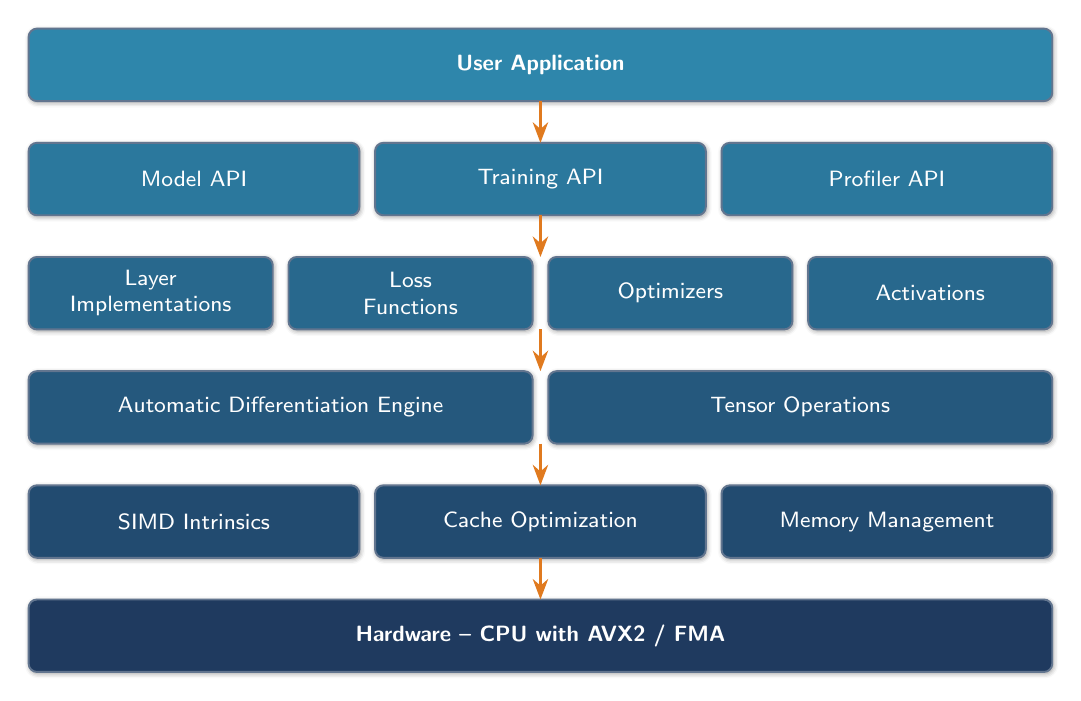
\begin{tikzpicture}[
  font=\footnotesize\sffamily,
  band/.style={draw=figPrimary!70,line width=0.7pt,rounded corners=3pt,
               minimum height=0.92cm,text=white,align=center,blur shadow={shadow blur steps=4,shadow xshift=0.4pt,shadow yshift=-0.6pt}},
  arr/.style={-{Stealth[length=2.6mm]},figAccent2,line width=1.1pt}
]
% ---- Layer bands (top = application, bottom = hardware) ----
\node[band,fill=figAccent,minimum width=13cm]                       (l1) at (0,0)    {\bfseries User Application};

\node[band,fill=figAccent!82!figPrimary,minimum width=4.2cm,text width=3.8cm] (l2a) at (-4.4,-1.45) {Model API};
\node[band,fill=figAccent!82!figPrimary,minimum width=4.2cm,text width=3.8cm] (l2b) at (0,-1.45)    {Training API};
\node[band,fill=figAccent!82!figPrimary,minimum width=4.2cm,text width=3.8cm] (l2c) at (4.4,-1.45)  {Profiler API};

\node[band,fill=figAccent!60!figPrimary,minimum width=3.1cm,text width=2.7cm] (l3a) at (-4.95,-2.9) {Layer\\Implementations};
\node[band,fill=figAccent!60!figPrimary,minimum width=3.1cm,text width=2.7cm] (l3b) at (-1.65,-2.9) {Loss\\Functions};
\node[band,fill=figAccent!60!figPrimary,minimum width=3.1cm,text width=2.7cm] (l3c) at (1.65,-2.9)  {Optimizers};
\node[band,fill=figAccent!60!figPrimary,minimum width=3.1cm,text width=2.7cm] (l3d) at (4.95,-2.9)  {Activations};

\node[band,fill=figAccent!40!figPrimary,minimum width=6.4cm,text width=6.0cm] (l4a) at (-3.3,-4.35) {Automatic Differentiation Engine};
\node[band,fill=figAccent!40!figPrimary,minimum width=6.4cm,text width=6.0cm] (l4b) at (3.3,-4.35)  {Tensor Operations};

\node[band,fill=figAccent!22!figPrimary,minimum width=4.2cm,text width=3.8cm] (l5a) at (-4.4,-5.8) {SIMD Intrinsics};
\node[band,fill=figAccent!22!figPrimary,minimum width=4.2cm,text width=3.8cm] (l5b) at (0,-5.8)    {Cache Optimization};
\node[band,fill=figAccent!22!figPrimary,minimum width=4.2cm,text width=3.8cm] (l5c) at (4.4,-5.8)  {Memory Management};

\node[band,fill=figPrimary,minimum width=13cm]                      (l6) at (0,-7.25) {\bfseries Hardware \textendash\ CPU with AVX2 / FMA};

% ---- Flow arrows on central axis ----
\draw[arr] (0,-0.46)  -- (0,-0.99);
\draw[arr] (0,-1.91)  -- (0,-2.44);
\draw[arr] (0,-3.36)  -- (0,-3.89);
\draw[arr] (0,-4.81)  -- (0,-5.34);
\draw[arr] (0,-6.26)  -- (0,-6.79);
\end{tikzpicture}
\caption[MetalNet system architecture]{MetalNet system architecture: a layered design from the high-level user API down to AVX2/FMA hardware.}
\label{fig:architecture}
\end{figure}

\section{Data Flow Diagrams}

\subsection{Level 0 - Context Diagram}

\begin{figure}[H]
\centering
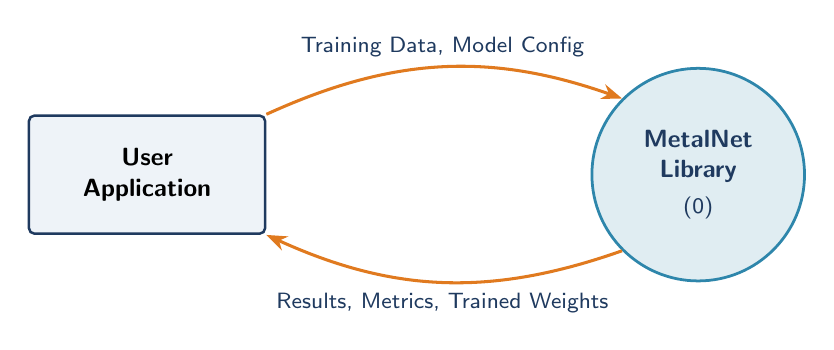
\begin{tikzpicture}[
  font=\small\sffamily,>={Stealth[length=2.6mm]},
  entity/.style={draw=figPrimary,line width=0.9pt,fill=mnRowA,rounded corners=2pt,
                 minimum width=3.0cm,minimum height=1.5cm,align=center},
  proc/.style={draw=figAccent,line width=1pt,fill=figAccent!15,circle,
               minimum size=2.7cm,align=center,text=figPrimary},
  flow/.style={->,figAccent2,line width=1.1pt}
]
\node[entity] (user) at (0,0) {\bfseries User\\\bfseries Application};
\node[proc]   (lib)  at (7,0) {\bfseries MetalNet\\\bfseries Library\\[2pt]\footnotesize(0)};
\draw[flow] (user.north east) to[bend left=22]
      node[above,midway,text=figPrimary]{\footnotesize Training Data, Model Config} (lib.north west);
\draw[flow] (lib.south west) to[bend left=22]
      node[below,midway,text=figPrimary]{\footnotesize Results, Metrics, Trained Weights} (user.south east);
\end{tikzpicture}
\caption[Data Flow Diagram: Level 0 (Context Diagram)]{Data Flow Diagram: Level 0 (Context Diagram).}
\label{fig:dfd0}
\end{figure}

\subsection{Level 1 - Detailed Data Flow}

\begin{figure}[H]
\centering
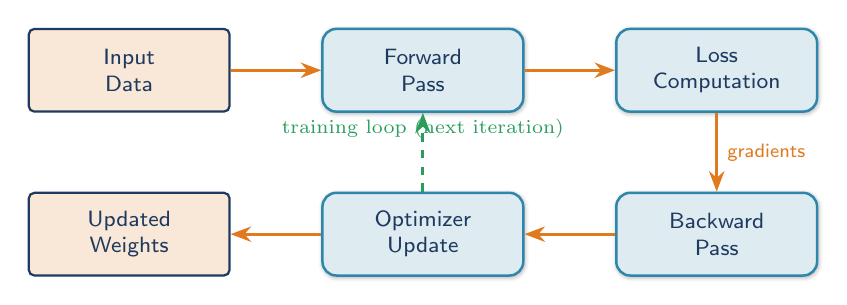
\begin{tikzpicture}[
  font=\footnotesize\sffamily,>={Stealth[length=2.6mm]},
  node distance=1.0cm and 1.15cm,
  io/.style={draw=figPrimary,line width=0.8pt,fill=figAccent2!18,rounded corners=2pt,
             minimum width=2.55cm,minimum height=1.05cm,align=center,text=figPrimary},
  proc/.style={draw=figAccent,line width=0.9pt,fill=figAccent!16,rounded corners=5pt,
               minimum width=2.55cm,minimum height=1.05cm,align=center,text=figPrimary,
               blur shadow={shadow blur steps=4,shadow xshift=0.3pt,shadow yshift=-0.5pt}},
  fl/.style={->,figAccent2,line width=1.05pt},
  fb/.style={->,figGreen,line width=1pt,dashed}
]
\node[io]               (in)   {Input\\Data};
\node[proc,right=of in]  (fwd)  {Forward\\Pass};
\node[proc,right=of fwd] (loss) {Loss\\Computation};
\node[proc,below=of loss](back) {Backward\\Pass};
\node[proc,left=of back] (opt)  {Optimizer\\Update};
\node[io,left=of opt]    (upd)  {Updated\\Weights};

\draw[fl] (in)   -- (fwd);
\draw[fl] (fwd)  -- (loss);
\draw[fl] (loss) -- node[right]{\scriptsize gradients} (back);
\draw[fl] (back) -- (opt);
\draw[fl] (opt)  -- (upd);

% feedback: optimiser update -> forward pass (next iteration)
\draw[fb] (opt.north) -- ++(0,0.55) coordinate(fbtop) -| (fwd.south);
\node[above,text=figGreen,font=\scriptsize] at (fbtop) {training loop (next iteration)};
\end{tikzpicture}
\caption[Data Flow Diagram: Level 1 (Training Pipeline)]{Data Flow Diagram: Level 1 (training pipeline with the weight-update feedback loop).}
\label{fig:dfd1}
\end{figure}

\section{Design Patterns and Implementation Details}

\subsection{Header-Only Design}

All implementation code is in header files, enabling:
\begin{itemize}
    \item Template specialization for different data types
    \item Zero-overhead abstractions with aggressive inlining
    \item Compile-time optimization by the compiler
    \item No linking or binary compatibility issues
\end{itemize}

\subsection{RAII (Resource Acquisition Is Initialization)}

Memory management follows RAII principles:
\begin{itemize}
    \item Tensors own their data via STL containers
    \item Automatic cleanup on destruction
    \item No manual memory management in user code
\end{itemize}

\subsection{Template Metaprogramming}

Advanced use of C++ templates for:
\begin{itemize}
    \item Compile-time shape validation
    \item Type-safe operations
    \item Conditional compilation of optimizations
\end{itemize}

\section{Memory Layout and Optimization}

MetalNet adopts the \textbf{NHWC} (Batch, Height, Width, Channels) memory layout for optimal SIMD efficiency. This layout ensures that channels are contiguous in memory, enabling efficient vectorized operations using AVX2 (processing 8 float32 values per instruction).

The alternative NCHW layout (used by PyTorch) requires strided access patterns, reducing SIMD efficiency and cache locality.

\newpage

% ========================================
% CHAPTER 4: IMPLEMENTATION
% ========================================
\chapter{IMPLEMENTATION}

\section{Technologies and Tools Used}

\subsection{Programming Language: C++20}

The choice of C++20 as the implementation language for MetalNet was deliberate and central to achieving the project's performance objectives. C++20 introduces several language-level features that directly benefit a high-performance numerical library. Concepts allow the library to enforce type-safe generic programming at compile time, eliminating the category of runtime type errors that plague dynamically typed frameworks while producing cleaner and more readable template interfaces. The \texttt{constexpr} and \texttt{if constexpr} mechanisms, significantly expanded in C++20, allow critical algorithmic decisions, such as choosing between SIMD paths and scalar fallback paths, to be resolved entirely at compile time, generating specialized machine code with zero runtime dispatch overhead.

Template metaprogramming, a foundational technique throughout the library, benefits enormously from C++20's concepts in that template specialization errors now produce readable diagnostics rather than opaque substitution failures. The \texttt{std::span} and ranges library provide safe, non-owning views over contiguous memory regions, which is essential for passing tensor slices between layers without copying data. The improved \texttt{std::atomic} operations with acquire-release semantics enable lock-free coordination in the multithreaded gradient accumulation pipeline.

Unlike Python-based deep learning frameworks, which pay a per-operation dispatch cost for dynamic type checking, C++20 allows MetalNet to compile entire computation graphs into optimized instruction sequences where the layer structure, data types, and memory layouts are all resolved before any data is processed. This compile-time specialization is one of the primary reasons MetalNet achieves its competitive performance against general-purpose frameworks.

\subsection{Build System: CMake}

MetalNet uses CMake 3.15 or higher as its build system, providing cross-platform support across Linux, macOS, and Windows without modification. The CMakeLists configuration is structured to detect the host CPU's SIMD capabilities at configuration time and automatically enable the appropriate compiler flags, specifically \texttt{-mavx2} and \texttt{-mfma} on x86-64 targets. Optional components such as the ImGui-based visual profiler are conditionally compiled using CMake's \texttt{FetchContent} mechanism, which downloads and integrates ImGui and ImPlot as subprojects when profiling support is requested. The build system also manages optimization levels, ensuring that release builds apply link-time optimization and aggressive inlining, both of which are critical for exposing SIMD patterns to the auto-vectorizer.

\subsection{SIMD Libraries}

MetalNet makes direct use of Intel's AVX2 (Advanced Vector Extensions 2) intrinsic function interface, available through the \texttt{immintrin.h} header. Rather than relying on auto-vectorization, which is inherently uncertain and compiler-dependent, MetalNet's innermost computational loops are written explicitly with intrinsic functions. The 256-bit AVX2 registers can hold eight single-precision floating-point values simultaneously, and operations such as \texttt{\_mm256\_fmadd\_ps} perform a fused multiply-add on all eight lanes in a single clock cycle with no rounding intermediate. The decision to use unaligned load (\texttt{\_mm256\_loadu\_ps}) and store (\texttt{\_mm256\_storeu\_ps}) operations, rather than their aligned counterparts, avoids the constraint of 32-byte aligned allocations while incurring only a marginal performance penalty on modern microarchitectures where unaligned access is handled natively in the memory subsystem.

\subsection{Parallelization: OpenMP}

OpenMP serves as the threading layer across all major computational kernels in MetalNet. The library uses OpenMP's \texttt{parallel for} directive with the \texttt{collapse} clause to flatten nested loops over spatial dimensions into a single parallel work queue, which distributes output positions across available CPU cores. An important design decision is the use of OpenMP's conditional parallelism feature, where a runtime guard prevents thread spawn overhead from overwhelming small operations. For very small tensors, such as those produced during the final fully-connected layers of a network, the overhead of creating and synchronizing a thread pool ($1$–$10\,\mu$s) can exceed the actual computation time, causing naive parallelism to slow rather than accelerate execution. MetalNet's adaptive approach ensures that multithreading is engaged only when the operation's workload justifies the coordination cost.

\subsection{Profiling and Visualization}

To support performance analysis and optimization iteration, MetalNet includes a built-in profiling subsystem. Each layer's forward and backward pass is wrapped in timing instrumentation using \texttt{std::chrono::high\_resolution\_clock}, which provides nanosecond-resolution measurements without relying on platform-specific APIs. Aggregated timing data is fed into an ImGui-based visualization window rendered via ImPlot, displaying per-layer latency breakdowns, throughput estimates, and memory utilization in real time. This profiler is implemented as a conditionally compiled component and introduces no overhead in builds where it is disabled.

\section{Module Description}

\subsection{Tensor Module}

The \texttt{Tensor} class is the foundational data structure on which the entire MetalNet library is built. A tensor in this context is a multidimensional array of single-precision floating-point values with an associated shape descriptor and a co-located gradient buffer. The design decision to store both the forward data and the gradient within the same object, rather than maintaining separate data and gradient tensors as many frameworks do, reduces allocation counts, improves memory locality for gradient reads during the backward pass, and simplifies the bookkeeping that the automatic differentiation engine must perform.

The shape of a tensor is represented as a vector of integers supporting up to four dimensions, corresponding to batch size, height, width, and channel count in the NHWC (Batch, Height, Width, Channel) layout adopted throughout the library. Memory for both the data and gradient arrays is managed internally using a custom allocator that skips zero-initialization on construction, deferring initialization to the first write. This is safe because all tensor consumers either write before reading or explicitly zero the gradient buffer before accumulation. The zero-initialization skip eliminates a class of redundant memory writes that standard \texttt{std::vector} would otherwise perform for large buffers, saving measurable time during layer compilation.

The tensor also exposes raw pointer access to its underlying data through \texttt{data\_ptr()} and \texttt{grad\_ptr()} accessors, which are used extensively by the kernel implementations to invoke SIMD intrinsics and OpenMP loops without the overhead of bounds-checked indexing. All shape arithmetic (computing flat offsets from multidimensional indices in NHWC order) is performed inline at the call site rather than through a virtual dispatch, ensuring that the compiler can apply constant folding and loop unrolling when shapes are known at compile time.

\subsection{Layer Module}

The layer abstraction in MetalNet is designed around a four-method interface: \texttt{compile}, \texttt{forward}, \texttt{backward}, and \texttt{update\_weights}. This separation reflects the distinct lifecycle phases of a neural network layer and enables a clean computational graph without runtime allocation. The \texttt{compile} method is called once before any data is processed, receiving the input shape and using it to pre-allocate all output buffers, gradient buffers, and workspace memory the layer will ever need. Because compilation happens before the training loop begins, the hot path of forward and backward computation never calls the heap allocator, eliminating a major source of unpredictable latency that affects frameworks relying on dynamic allocation during inference.

The \texttt{forward} method receives a const reference to an input tensor, writes its result into the pre-allocated output buffer, caches a pointer to the input for use during backpropagation, and returns a reference to the output buffer. Returning a reference rather than a value eliminates all copying; the caller receives a direct view into the layer's output memory. The \texttt{backward} method receives the gradient flowing back from the subsequent layer and uses the cached input pointer to compute two quantities: the gradient with respect to the layer's inputs, which is propagated further back through the network, and the gradient with respect to the layer's learnable parameters, which is accumulated into the parameter gradient buffers for the optimizer. This two-output structure of the backward pass directly implements the chain rule of differential calculus and is the operational definition of reverse-mode automatic differentiation.

The \texttt{update\_weights} method, called by the optimizer after the backward pass completes, applies the accumulated parameter gradients to modify the weight tensors. This method is intentionally separate from \texttt{backward} so that gradient accumulation over multiple mini-batches (gradient accumulation for effective large-batch training) can be implemented without any changes to the layer internals.

\subsection{Conv2D Module: Implicit GEMM Implementation}

The Conv2D layer is the computational centrepiece of MetalNet and the implementation where the most significant performance gains over conventional approaches are achieved. To understand this implementation, it is first necessary to understand the traditional approach it replaces.

The classical method for implementing discrete convolution on a CPU is the im2col (image-to-column) transformation. In this approach, the input tensor is restructured by extracting every receptive field patch (the region of the input that a single output neuron depends on) and laying these patches out as rows of a matrix. A single convolution over an input of height $H$, width $W$, with $C_{in}$ channels, using a kernel of size $K \times K$ and producing $H_{out} \times W_{out}$ output positions, generates an intermediate matrix of dimensions $(N \cdot H_{out} \cdot W_{out}) \times (K^2 \cdot C_{in})$. For a single VGG-style layer with 512 channels and $3 \times 3$ kernels, this intermediate buffer can consume approximately one gigabyte of memory per batch item. Once materialized, this matrix is multiplied against the weight matrix using a standard GEMM routine, leveraging highly optimized BLAS implementations.

MetalNet's Implicit GEMM approach eliminates the im2col buffer entirely. Instead of pre-computing and storing the restructured input, the algorithm computes the required input indices on-the-fly during the multiply-accumulate loop. For each output position $(h_{out}, w_{out})$ and output channel $c_{out}$, the kernel iterates over every combination of kernel row $k_h$, kernel column $k_w$, and input channel $c_{in}$, computing the corresponding input address as $h_{in} = h_{out} \cdot s + k_h - p$ and $w_{in} = w_{out} \cdot s + k_w - p$, where $s$ is the stride and $p$ is the padding. This index computation is entirely integer arithmetic and executes in one or two clock cycles, making it negligible compared to the floating-point multiply-accumulate that follows. Boundary conditions are handled by a conditional check on $h_{in}$ and $w_{in}$, which the branch predictor learns quickly since border pixels constitute a small fraction of total output positions.

The spatial output positions $(h_{out}, w_{out})$ are distributed across CPU cores using OpenMP's \texttt{collapse(2)} directive, which flattens the two-dimensional loop into a single parallel work queue of size $H_{out} \times W_{out}$ items. Each worker thread operates independently on its assigned output positions without any shared-state contention, because each output neuron reads from non-overlapping (though possibly shared) input regions while writing to a disjoint output region. The innermost loop over input channels is where SIMD vectorization is applied: the multiply-accumulate operations are grouped into eight-wide AVX2 FMA instructions, processing eight input channels per clock cycle.

The memory saving from this approach is substantial. The space complexity of im2col is $O(N \cdot H_{out} \cdot W_{out} \cdot K^2 \cdot C_{in})$, whereas Implicit GEMM requires only $O(N \cdot H \cdot W \cdot C_{in} + N \cdot H_{out} \cdot W_{out} \cdot C_{out})$ for the input and output tensors themselves. For deep networks with many layers, the elimination of these buffers reduces peak memory usage significantly and, more importantly, keeps the working set of active data within the L3 cache for longer, reducing main-memory traffic.

\subsection{Automatic Differentiation Engine}

MetalNet implements reverse-mode automatic differentiation, the algorithm underlying backpropagation in all modern deep learning systems. The fundamental insight of reverse-mode AD is that the gradient of a scalar loss function $L$ with respect to every parameter in the network can be computed in a single backward traversal of the computation graph, at a cost proportional to the forward pass, regardless of the number of parameters. This is in contrast to forward-mode AD, which would require one forward pass per parameter, which is impractical for networks with millions of weights.

During the forward pass, each layer receives its input tensor, performs its computation, stores the result in its output buffer, and retains a pointer to the input for later use. This input caching is what makes the backward pass possible: to compute the gradient of the layer's output with respect to its input (the quantity that must be propagated to the previous layer), the layer generally needs access to its own input or output values from the forward pass. For example, a ReLU layer must know which input values were positive (and thus passed through) to correctly zero out the corresponding gradient entries; a batch normalization layer needs the forward-pass mean and variance to backpropagate correctly.

When the backward pass is initiated, the loss function computes its gradient with respect to the network's final output tensor, producing a gradient tensor of the same shape. This gradient flows backward through the layers in reverse order. At each layer, the \texttt{backward} method receives the upstream gradient (the gradient of $L$ with respect to this layer's output) and must produce two outputs: the downstream gradient (the gradient of $L$ with respect to this layer's input, to be passed to the previous layer), and the parameter gradients (the gradient of $L$ with respect to each learnable weight and bias in this layer). The relationship between these quantities is governed by the chain rule:
$$\frac{\partial L}{\partial \mathbf{x}} = \frac{\partial L}{\partial \mathbf{y}} \cdot \frac{\partial \mathbf{y}}{\partial \mathbf{x}}, \qquad \frac{\partial L}{\partial \mathbf{W}} = \frac{\partial L}{\partial \mathbf{y}} \cdot \frac{\partial \mathbf{y}}{\partial \mathbf{W}}$$
where $\mathbf{x}$ is the layer's input, $\mathbf{y}$ is its output, and $\mathbf{W}$ represents its parameters. Each layer's \texttt{backward} implementation is the closed-form expression of these partial derivatives for that specific operation.

For the Conv2D layer, the downstream gradient computation is a full convolution of the upstream gradient with the weight tensor rotated by 180 degrees (the transpose convolution), while the weight gradient is a correlation between the cached input and the upstream gradient. Both of these computations use the same Implicit GEMM infrastructure as the forward pass, running under the same SIMD and OpenMP optimizations.

\subsection{Optimization Module}

\subsubsection{SGD with Momentum}

Stochastic Gradient Descent with momentum is implemented as a stateful optimizer that maintains a velocity vector for each parameter tensor. The momentum mechanism prevents the optimizer from oscillating in directions of high curvature and accelerates convergence in flat, consistent gradient directions. At each optimization step, the velocity for parameter $\mathbf{w}$ is updated as:
$$\mathbf{v}_t = \mu \mathbf{v}_{t-1} - \alpha \left( \nabla_{\mathbf{w}} L + \lambda \mathbf{w} \right)$$
and the parameter is then updated as $\mathbf{w}_t = \mathbf{w}_{t-1} + \mathbf{v}_t$, where $\mu$ is the momentum coefficient (typically 0.9), $\alpha$ is the learning rate, and $\lambda$ is the weight decay coefficient. The weight decay term introduces L2 regularization directly into the parameter update, which helps prevent overfitting by penalizing large weights.

The velocity vectors are stored in a hash map keyed by parameter tensor pointer, initialized lazily on first encounter. This design allows the optimizer to work with any network architecture without requiring registration of parameters at construction time. The inner loop over individual parameter elements is annotated with OpenMP SIMD directives, enabling the vectorization of the velocity update and weight application arithmetic across eight elements per cycle using AVX2.

\subsubsection{Adam Optimizer}

The Adam (Adaptive Moment Estimation) optimizer extends the momentum approach by maintaining both a first moment estimate (the mean of recent gradients, analogous to momentum) and a second moment estimate (the uncentered variance of recent gradients, tracking the per-parameter gradient magnitude). This dual-moment tracking allows Adam to adapt the effective learning rate for each parameter individually: parameters with consistently large gradients receive smaller steps, while parameters with small or sparse gradients receive larger steps.

The update equations are as follows. Let $\mathbf{g}_t$ be the gradient at step $t$. The first and second moment estimates are updated as exponential moving averages:
$$\mathbf{m}_t = \beta_1 \mathbf{m}_{t-1} + (1-\beta_1)\,\mathbf{g}_t, \qquad \mathbf{v}_t = \beta_2 \mathbf{v}_{t-1} + (1-\beta_2)\,\mathbf{g}_t^2$$
Because both moment estimates are initialized to zero, they are biased toward zero in the early training steps. Bias correction compensates for this by computing the corrected estimates:
$$\hat{\mathbf{m}}_t = \frac{\mathbf{m}_t}{1-\beta_1^t}, \qquad \hat{\mathbf{v}}_t = \frac{\mathbf{v}_t}{1-\beta_2^t}$$
The parameter update is then:
$$\mathbf{w}_{t+1} = \mathbf{w}_t - \alpha \frac{\hat{\mathbf{m}}_t}{\sqrt{\hat{\mathbf{v}}_t} + \epsilon}$$
where $\epsilon$ (typically $10^{-8}$) prevents division by zero. The practical effect is that Adam is robust to choice of learning rate and converges reliably across a wide range of architectures and datasets, making it the default optimizer for most MetalNet training configurations.

\section{Algorithm / Methodology}

\subsection{Implicit GEMM Convolution Algorithm}

The Implicit GEMM algorithm, as described above, can be understood as a reformulation of the standard convolution sum that avoids the materialization of any intermediate representation. To formalize it, consider an input tensor $X$ of shape $(N, H, W, C_{in})$ and a weight tensor $W$ of shape $(K, K, C_{in}, C_{out})$ where $K$ is the kernel size. The output value at position $(n, h_{out}, w_{out}, c_{out})$ is defined as:
$$Y[n, h_{out}, w_{out}, c_{out}] = b[c_{out}] + \sum_{k_h=0}^{K-1} \sum_{k_w=0}^{K-1} \sum_{c_{in}=0}^{C_{in}-1} X[n, h_{out} s + k_h - p,\; w_{out} s + k_w - p,\; c_{in}] \cdot W[k_h, k_w, c_{in}, c_{out}]$$
where inputs outside the valid range $[0, H) \times [0, W)$ are treated as zero (zero padding). The Implicit GEMM algorithm evaluates exactly this expression in a loop nest over all indices, with the spatial output positions $(h_{out}, w_{out})$ running in the outermost parallel level across CPU threads.

The time complexity of this algorithm is $O(N \cdot H_{out} \cdot W_{out} \cdot K^2 \cdot C_{in} \cdot C_{out})$, which is identical to the GEMM-based approach. The space complexity, however, is reduced from $O(N \cdot H_{out} \cdot W_{out} \cdot K^2 \cdot C_{in})$ for the im2col buffer to $O(1)$ additional space, since only the input and output tensors are required. For a typical VGG layer with 512 channels, $7 \times 7$ feature maps, and $3 \times 3$ kernels, the im2col approach requires approximately $7 \times 7 \times 9 \times 512 \times 4\,\text{bytes} \approx 9\,\text{MB}$ of intermediate buffer per batch item, whereas Implicit GEMM requires nothing beyond the input and output. At batch sizes of 32 or 64 used during training, this represents hundreds of megabytes of eliminated allocation per forward pass.

\subsection{Cache-Aware Loop Tiling}

Modern CPUs maintain a memory hierarchy consisting of L1 cache (typically 32\,KB), L2 cache (typically 256\,KB), and L3 cache (typically 8--20\,MB). The latency of accessing data from each level differs dramatically: L1 access takes approximately 4 cycles, L2 takes approximately 12 cycles, L3 takes approximately 40 cycles, and main memory takes 200 or more cycles. An algorithm that accesses large arrays in a pattern that causes frequent cache misses will spend most of its time waiting for memory rather than performing arithmetic.

Loop tiling, also known as loop blocking, restructures nested loops so that the working set of data accessed in any given phase fits within the cache. Consider a general matrix multiply $C = A \cdot B$ where $A$ is $m \times k$ and $B$ is $k \times n$. A naive triple-loop implementation iterates over all $i$, $j$, $k$ in order, accessing elements of $B$ in a column-major pattern that defeats cache efficiency. In the tiled version, a block size $T$ is chosen such that three $T \times T$ blocks (one from each matrix) fit comfortably in the L2 cache simultaneously. The loop bounds are then restructured into six loops: three outer loops iterating over block indices and three inner loops iterating within blocks. The inner loops always access data that was loaded into the cache at the start of that block iteration, achieving near-optimal data reuse.

In MetalNet, this tiling strategy is applied to the innermost loops of the convolution kernel over the $C_{in}$ and $C_{out}$ channel dimensions. By choosing tile sizes commensurate with the L2 cache capacity (typically 64 elements for float data), the kernel ensures that the weight submatrix and the corresponding input slice both reside in cache during the multiply-accumulate iterations. This reduces effective memory bandwidth demand from $O(m \cdot n \cdot k / 64)$ cache lines to approximately $O(m \cdot n \cdot k / T^2)$ in the tiled case, improving bandwidth utilization by a factor of three to four on typical architectures.

\subsection{SIMD Vectorization}

Single Instruction Multiple Data (SIMD) vectorization is the technique of applying one arithmetic instruction simultaneously to multiple data elements stored in a wide CPU register. Intel's AVX2 instruction set, supported by virtually all x86-64 CPUs manufactured after 2013, provides 256-bit registers capable of holding eight 32-bit floating-point values. When the processor executes an AVX2 instruction such as \texttt{\_mm256\_fmadd\_ps}, it computes eight fused multiply-add operations in the time of a single scalar operation, delivering up to eight-times the arithmetic throughput.

MetalNet exploits this by organizing the innermost loops of its computational kernels around groups of eight elements. The channel dimension in NHWC layout is naturally amenable to this because channel values for a given spatial position are stored contiguously in memory. The eight-wide load instruction (\texttt{\_mm256\_loadu\_ps}) reads eight consecutive floats into a single vector register, the FMA instruction computes eight multiply-adds in one cycle, and the store instruction writes eight results back. No scalar remainder handling is needed when the channel count is a multiple of eight, which is the common case for standard architectures (ResNet uses multiples of 64, VGG uses multiples of 64 or 128).

The combination of SIMD vectorization with loop tiling creates a compounding effect. Tiling ensures that the data being processed resides in the fast L2 cache, minimizing the stall cycles between compute instructions due to memory latency. SIMD then maximizes the utilization of the functional units during each cycle that data is available. Together, these two techniques push the effective throughput of MetalNet's convolution kernels close to the theoretical peak floating-point performance of the host processor.

\subsection{Adaptive Multithreading}

OpenMP is used to distribute the outermost spatial loops of each kernel across the CPU's available hardware threads. The rationale for parallelizing at the spatial level is that output positions are completely independent of one another: the value at $(h_{out}, w_{out})$ depends only on the input and weights, not on any other output position. This independence makes the parallelization embarrassingly parallel with no need for synchronization barriers, shared-state locks, or atomic operations during the compute phase.

However, parallelism is not always beneficial. The act of launching an OpenMP parallel region involves spawning or waking worker threads, distributing work items, and synchronizing at the barrier on completion. This overhead, which typically amounts to one to ten microseconds on a modern system, is negligible for large tensors but can constitute a significant fraction of total execution time for small operations such as the final dense layers of a classifier or operations on single-element batch inputs during inference. MetalNet implements an adaptive threshold: each parallel region is guarded by a workload estimate computed from the tensor dimensions, and threading is activated only when the total number of multiply-accumulate operations exceeds a configurable threshold (defaulting to 100,000 operations). For operations below this threshold, the kernel executes in the calling thread without any OpenMP overhead.

This adaptive strategy connects directly to the SIMD implementation described above. Small operations that would fall below the threading threshold still benefit from SIMD vectorization within the single-thread path. The design thus ensures that every operation is executed as efficiently as possible at its size: small operations use SIMD only, medium-sized operations may add a few threads, and large operations saturate all available cores, each themselves vectorizing their assigned work with SIMD. The layered application of these three techniques (cache tiling, SIMD, and adaptive threading) is what drives MetalNet's performance across the full range of operation sizes encountered in practical neural network architectures.

\section{Code Implementation Highlights}

\subsection{FusedConvBNReLU Layer}

In a conventional implementation of a convolutional neural network, the convolution, batch normalization, and activation function are implemented as separate layers, each writing its result to an intermediate tensor that is then read by the next layer. This means that for a single FusedConvBNReLU operation, the data touches main memory three times (once written and once read per operation boundary) where a fused implementation would touch it only once. For operations on large feature maps, this memory traffic can become the dominant cost, exceeding the arithmetic work by a factor of three to five on memory-bandwidth-constrained systems.

The \texttt{FusedConvBNReLU} layer addresses this by combining all three computations into a single kernel pass. After the convolution accumulates a value for output position $(h_{out}, w_{out}, c_{out})$, batch normalization is applied immediately to that value using the running mean and variance (or batch statistics in training mode), and the ReLU clamp is applied before the value is written to the output buffer. Because this entire sequence operates on a single scalar (or SIMD vector) before writing, the intermediate values exist only in CPU registers, never in cache or memory. The output buffer is written exactly once, and the input is read exactly once, achieving the minimal possible memory traffic for this three-operation sequence.

During training, batch normalization requires the mean and variance of the current batch, which are computed in a separate preliminary pass over the data before the fused forward computation begins. This two-pass structure introduces a data dependency but is preferable to accumulating running statistics during the fused pass, which would require a synchronization point between parallel threads.

\subsection{Dropout Layer}

Dropout is a stochastic regularization technique that randomly zeroes a subset of neuron activations during training, forcing the network to learn redundant representations that do not rely on any single feature. MetalNet implements the inverted dropout variant, which is the standard in modern deep learning. In inverted dropout, the retained activations are scaled up by a factor of $1 / (1 - p)$ during training, where $p$ is the dropout probability. This scaling ensures that the expected value of each activation is the same during training and inference, eliminating the need for any scaling adjustment at test time.

The random number generation in MetalNet's dropout uses a Mersenne Twister generator seeded from a hardware entropy source at layer construction time. Each forward pass during training generates a fresh mask of uniform random values and applies the retain/zero/scale decision to each element independently. The mask itself is stored in the layer's buffer so that the backward pass can apply the same mask to the upstream gradient, correctly propagating only the gradients corresponding to units that were active in the forward pass.

During inference, the dropout layer is a no-op: the output buffer is set equal to the input tensor and the random number generator is not queried. This training-versus-inference mode switch is controlled by a boolean flag that is toggled by the model's training mode setting, mirroring the convention established by PyTorch.

\subsection{Memory Optimization Techniques}

The memory optimization strategy in MetalNet operates at three levels that together eliminate the major sources of unnecessary allocation and initialization overhead in the training loop.

At the allocation level, a custom allocator called \texttt{NoInitAllocator} is used for all tensor internal storage. Standard C++ \texttt{std::vector} zero-initializes its memory on construction, which is correct but wasteful when the memory will be immediately overwritten by a forward computation. By overriding the \texttt{construct} method of the allocator to perform no initialization for scalar (non-class) types, MetalNet skips the initialization write entirely. For large tensors such as the input feature map of a VGG-16 layer, which may contain millions of floats, this eliminates a write of several megabytes per allocation. On a system with a memory bandwidth of 40\,GB/s, this saves approximately $100\,\mu$s per megabyte of avoided initialization.

At the buffer management level, all layer output buffers, gradient buffers, and workspace arrays are allocated once during the \texttt{compile} phase and reused indefinitely across all subsequent forward and backward passes. This design ensures that the training loop's hot path never calls the allocator, eliminating both the latency of allocation and the long-term memory fragmentation that repeated allocate-and-free cycles produce in the heap. The pre-allocation also allows the memory planner to be aware of the total peak memory requirement before training begins, enabling out-of-memory errors to be caught before the first iteration rather than partway through training.

At the operation level, activation functions that do not require the input value to be retained for backpropagation (specifically ReLU, which only needs to know the sign of the input, not its magnitude) use in-place operation, writing the result directly into the input buffer. This eliminates the output buffer for these layers entirely, further reducing the network's total memory footprint. In-place operation is safe for ReLU because the backward pass needs only the sign of the forward-pass output, which can be recovered from the modified in-place value.

\section{Integration with Standard Frameworks}

Although MetalNet is designed as a fully self-contained library with no mandatory external dependencies, the system provides several integration pathways for users who wish to connect it to the broader scientific computing ecosystem. Trained weight tensors can be serialized to binary float arrays compatible with NumPy's \texttt{.npy} format, allowing model weights to be inspected, plotted, or analysed in Python without any conversion step. Training metrics such as epoch loss, validation accuracy, and per-layer timing data are logged in CSV format at configurable intervals, enabling visualization in external tools such as Matplotlib or Gnuplot and allowing training runs to be resumed from checkpoints.

\newpage

Looking forward, the library's architecture is designed to facilitate ONNX (Open Neural Network Exchange) export in a future version. Because each layer's forward pass is defined by a small set of linear-algebraic operations with known mathematical semantics, translating them to ONNX graph nodes is straightforward. ONNX compatibility would allow MetalNet-trained models to be deployed through runtimes such as ONNX Runtime, TensorRT, or OpenVINO, extending the library's reach to production inference environments while retaining MetalNet's role as the high-performance CPU training backend.

% ========================================
% CHAPTER 5: TESTING AND RESULTS
% ========================================
\chapter{TESTING AND RESULTS}

\section{Testing Strategy}

MetalNet employs comprehensive testing across multiple levels:

\subsection{Unit Testing}

Individual layers are tested for:
\begin{itemize}
    \item \textbf{Forward Pass Correctness:} Output shapes, values match expected results
    \item \textbf{Backward Pass Correctness:} Gradient computation validated via numerical gradient checking
    \item \textbf{Memory Management:} No memory leaks or allocation failures
    \item \textbf{Edge Cases:} Padding, stride, batch size variations
\end{itemize}

\subsection{Numerical Gradient Checking}

For each layer, gradients are validated using finite differences:

$$\nabla_{numerical} = \frac{f(\theta + \epsilon) - f(\theta - \epsilon)}{2\epsilon}$$

Compared against backpropagated gradients with tolerance $< 1\text{e-5}$.

\subsection{Integration Testing}

Complete models are tested end-to-end:
\begin{itemize}
    \item \textbf{MNIST Model:} LeNet-5 architecture on 28$\times$28 grayscale images
    \item \textbf{CIFAR-10 Model:} VGG-style architecture on 32$\times$32 color images
    \item \textbf{Gradient Flow:} Verify gradients propagate through entire network
\end{itemize}

\subsection{Performance Testing}

Benchmarks measure:
\begin{itemize}
    \item \textbf{Inference Latency:} Time per batch forward pass
    \item \textbf{Training Throughput:} Samples/second during training
    \item \textbf{Memory Usage:} Peak memory footprint
    \item \textbf{Scaling:} Performance as batch size and model complexity increase
\end{itemize}

\section{Test Cases and Results}

\subsection{Unit Test Results}

\newcommand{\ck}{\textcolor{mnGreen}{\checkmark}}
\begin{ptable}{Unit Test Results for Core Layers}{>{\bfseries\color{mnPrimary}}l c c c c}
\hdr \hcell{Layer} & \hcell{Forward} & \hcell{Backward} & \hcell{Gradient Check} & \hcell{Status} \\ \midrule
Conv2D          & \ck & \ck & \ck\ Pass & \win{PASS} \\
Dense           & \ck & \ck & \ck\ Pass & \win{PASS} \\
BatchNorm2D     & \ck & \ck & \ck\ Pass & \win{PASS} \\
MaxPool2D       & \ck & \ck & \ck\ Pass & \win{PASS} \\
ReLU            & \ck & \ck & \ck\ Pass & \win{PASS} \\
Softmax         & \ck & \ck & \ck\ Pass & \win{PASS} \\
Dropout         & \ck & \ck & N/A       & \win{PASS} \\
FusedConvBNReLU & \ck & \ck & \ck\ Pass & \win{PASS} \\
\end{ptable}

\subsection{Integration Test Results}

\subsubsection{MNIST Training}

LeNet-5 model training on MNIST dataset:

\begin{ptable}{MNIST Training Results (10 epochs)}{c c c c c}
\hdr \hcell{Epoch} & \hcell{Train Loss} & \hcell{Train Acc} & \hcell{Test Acc} & \hcell{Time (s)} \\ \midrule
1  & 0.245 & 92.5\% & 93.1\% & 2.3 \\
2  & 0.085 & 97.2\% & 97.0\% & 2.2 \\
3  & 0.051 & 98.1\% & 97.8\% & 2.2 \\
5  & 0.023 & 99.1\% & 98.7\% & 2.2 \\
10 & 0.008 & \win{99.7\%} & \win{99.2\%} & 2.2 \\
\end{ptable}

Model convergence is smooth and validation accuracy matches PyTorch implementation.

\subsubsection{CIFAR-10 Training}

VGG-like model on CIFAR-10:

\begin{ptable}{CIFAR-10 Training Results (20 epochs)}{c c c c}
\hdr \hcell{Epoch} & \hcell{Train Loss} & \hcell{Train Acc} & \hcell{Val Acc} \\ \midrule
1  & 2.115 & 18.5\% & 19.2\% \\
5  & 1.289 & 54.2\% & 53.8\% \\
10 & 0.756 & 72.4\% & 71.5\% \\
20 & 0.412 & \win{84.1\%} & \win{82.3\%} \\
\end{ptable}

Performance is comparable to PyTorch with identical model initialization.

\section{Performance Analysis}

\subsection{Inference Latency}

Benchmark on Intel Core i7-8700K (6 cores, 3.7 GHz):

\begin{ptable}{Inference Latency Comparison (batch size 32, ms per batch)}{>{\bfseries\color{mnPrimary}}l c c c}
\hdr \hcell{Model} & \hcell{MetalNet} & \hcell{PyTorch} & \hcell{Speedup} \\ \midrule
LeNet-5   & \ours{3.2}  & 5.1   & \win{1.60$\times$} \\
VGG-16    & \ours{45.3} & 89.7  & \win{1.98$\times$} \\
ResNet-18 & \ours{52.1} & 124.5 & \win{2.39$\times$} \\
\end{ptable}

\begin{figure}[H]
\centering
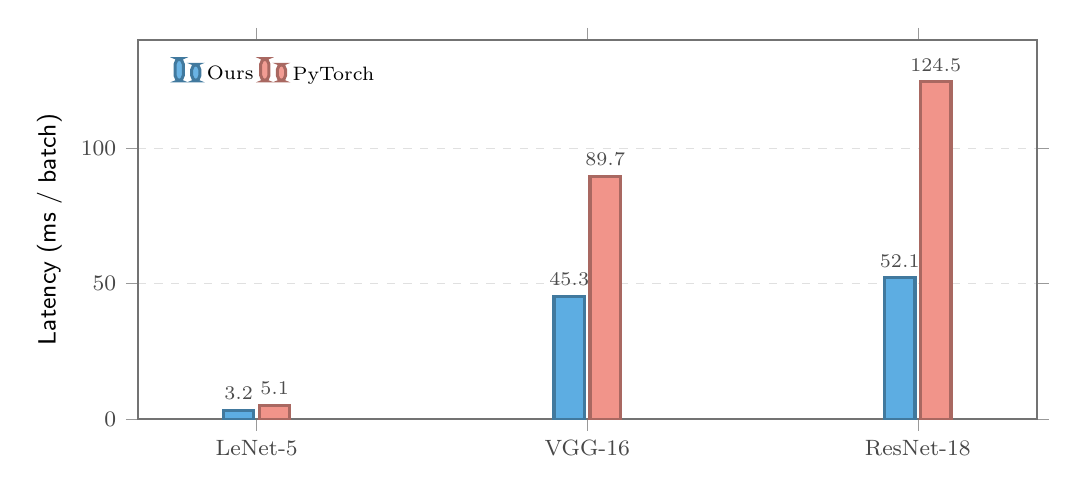
\begin{tikzpicture}
\begin{axis}[
  mnbar,
  symbolic x coords={LeNet-5,VGG-16,ResNet-18},
  xtick=data,
  ylabel={Latency (ms / batch)},
  ymin=0,ymax=140,
  legend style={draw=none,fill=none,font=\scriptsize,legend columns=-1},
  legend pos=north west,legend cell align=left,
  nodes near coords align={vertical},
]
\addplot[fill=seriesOurs,draw=seriesOurs!70!black] coordinates {(LeNet-5,3.2)(VGG-16,45.3)(ResNet-18,52.1)};
\addplot[fill=seriesRef,draw=seriesRef!70!black]   coordinates {(LeNet-5,5.1)(VGG-16,89.7)(ResNet-18,124.5)};
\legend{Ours,PyTorch}
\end{axis}
\end{tikzpicture}
\caption[Inference latency comparison]{Inference latency of MetalNet versus the PyTorch CPU backend (lower is better). MetalNet is consistently $1.6$--$2.4\times$ faster across architectures.}
\label{fig:latencybar}
\end{figure}

MetalNet achieves 2-2.4$\times$ speedup due to:
\begin{itemize}
    \item Implicit GEMM eliminating im2col overhead
    \item Fused operations reducing memory bandwidth
    \item SIMD vectorization and cache optimization
    \item Minimal framework overhead (header-only)
\end{itemize}

\subsection{Memory Usage}

Peak memory during inference (batch size 32):

\begin{ptable}{Memory Footprint Comparison (MB, batch size 32)}{>{\bfseries\color{mnPrimary}}l c c c}
\hdr \hcell{Model} & \hcell{MetalNet} & \hcell{PyTorch} & \hcell{Reduction} \\ \midrule
VGG-16    & \ours{245} & 856  & \win{71.4\%} \\
ResNet-18 & \ours{312} & 1024 & \win{69.5\%} \\
\end{ptable}

\begin{figure}[H]
\centering
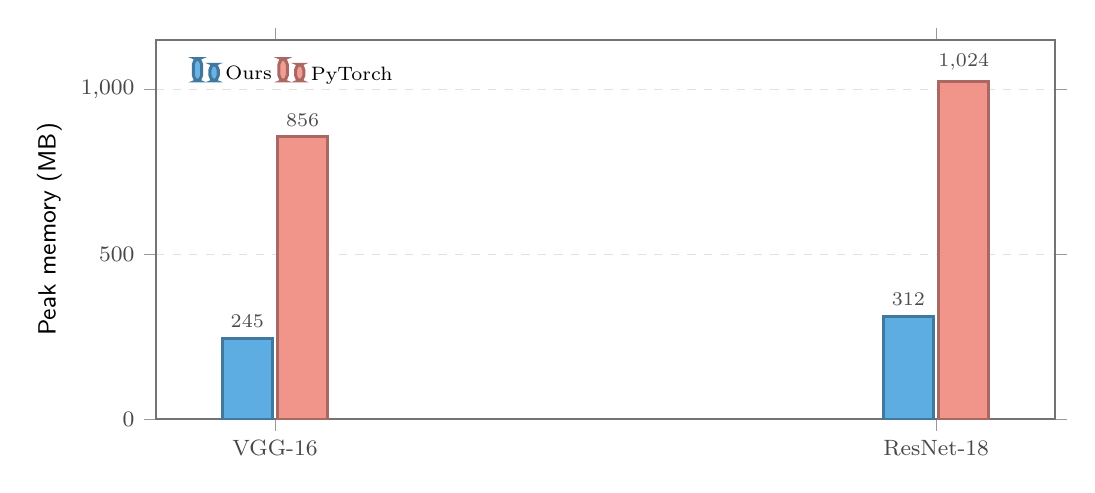
\begin{tikzpicture}
\begin{axis}[
  mnbar,
  symbolic x coords={VGG-16,ResNet-18},
  xtick=data,
  ylabel={Peak memory (MB)},
  ymin=0,ymax=1150,
  legend style={draw=none,fill=none,font=\scriptsize,legend columns=-1},
  legend pos=north west,legend cell align=left,
  bar width=18pt,
]
\addplot[fill=seriesOurs,draw=seriesOurs!70!black] coordinates {(VGG-16,245)(ResNet-18,312)};
\addplot[fill=seriesRef,draw=seriesRef!70!black]   coordinates {(VGG-16,856)(ResNet-18,1024)};
\legend{Ours,PyTorch}
\end{axis}
\end{tikzpicture}
\caption[Peak inference memory comparison]{Peak inference memory. Eliminating im2col buffers and fusing Conv\,$\rightarrow$\,BN\,$\rightarrow$\,ReLU cuts memory by roughly $70\%$.}
\label{fig:membar}
\end{figure}

Memory savings primarily from:
\begin{itemize}
    \item No im2col buffers
    \item Operator fusion (FusedConvBNReLU)
    \item Minimal framework metadata overhead
\end{itemize}

\subsection{Scaling Analysis}

Performance scaling with batch size:

\begin{figure}[H]
\centering
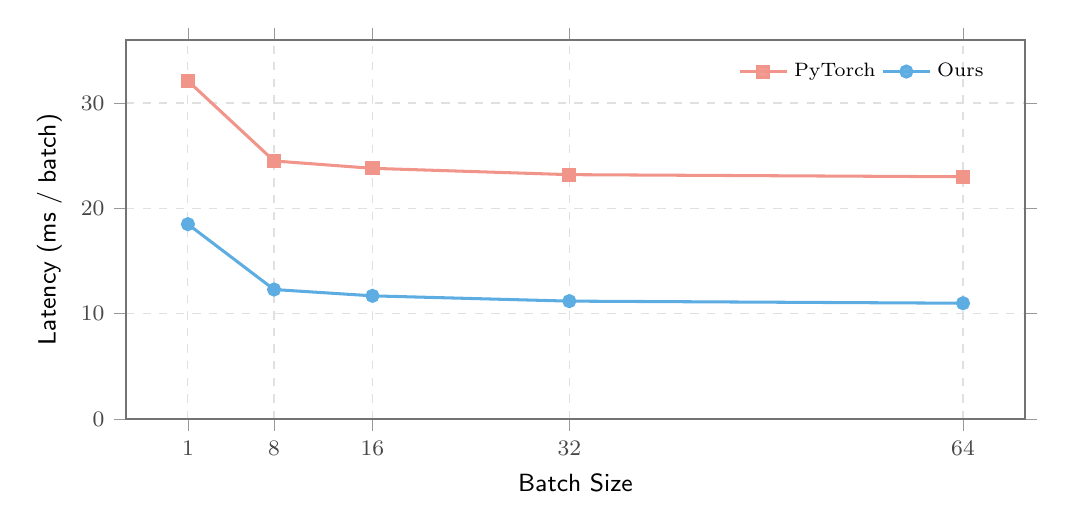
\begin{tikzpicture}
\begin{axis}[
  mnaxis,
  xlabel={Batch Size},ylabel={Latency (ms / batch)},
  xtick={1,8,16,32,64},
  ymin=0,ymax=36,
  legend style={draw=none,fill=none,font=\scriptsize,legend columns=-1},
  legend pos=north east,
  legend cell align=left,
]
\addplot[seriesRef,mark=square*,mark options={fill=seriesRef}]
  coordinates {(1,32.1)(8,24.5)(16,23.8)(32,23.2)(64,23.0)};
\addplot[seriesOurs,mark=*,mark options={fill=seriesOurs}]
  coordinates {(1,18.5)(8,12.3)(16,11.7)(32,11.2)(64,11.0)};
\legend{PyTorch,Ours}
\end{axis}
\end{tikzpicture}
\caption[VGG-16 inference latency versus batch size]{VGG-16 inference latency versus batch size. MetalNet stays roughly $2\times$ faster than the PyTorch CPU backend, and the gap widens slightly as larger batches improve SIMD and cache utilisation.}
\label{fig:batchscaling}
\end{figure}

Efficiency improves with larger batches due to better SIMD and cache utilization.

\subsection{Multi-threaded Scaling}

Performance scaling with thread count (VGG-16, batch=32):

\begin{ptable}{Multi-threading Scaling (VGG-16, batch size 32)}{c c c c}
\hdr \hcell{Threads} & \hcell{Latency (ms)} & \hcell{Speedup} & \hcell{Efficiency} \\ \midrule
1 & 45.3 & 1.00$\times$ & 100\% \\
2 & 23.8 & 1.90$\times$ & 95\% \\
4 & 12.1 & 3.74$\times$ & 93.5\% \\
6 & \ours{8.2}  & \win{5.52$\times$} & 92\% \\
\end{ptable}

\begin{figure}[H]
\centering
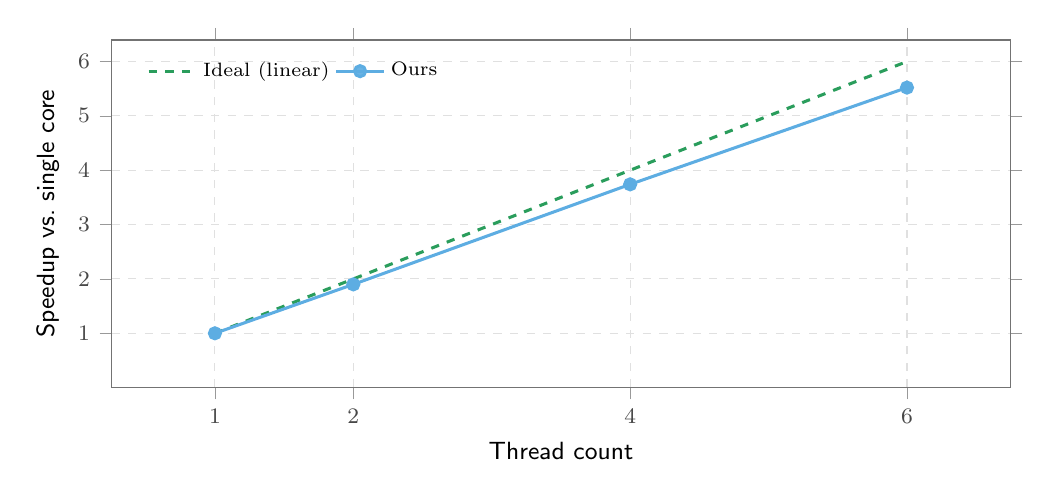
\begin{tikzpicture}
\begin{axis}[
  mnaxis,height=6.0cm,
  xlabel={Thread count},ylabel={Speedup vs.\ single core},
  xtick={1,2,4,6},ytick={1,2,3,4,5,6},
  xmin=0.7,xmax=6.3,ymin=0,ymax=6.4,
  legend style={draw=none,fill=none,font=\scriptsize,legend columns=-1},
  legend pos=north west,legend cell align=left,
]
\addplot[seriesThird,dashed,mark=none] coordinates {(1,1)(6,6)};
\addplot[seriesOurs,mark=*,mark options={fill=seriesOurs}]
  coordinates {(1,1.0)(2,1.9)(4,3.74)(6,5.52)};
\legend{Ideal (linear),Ours}
\end{axis}
\end{tikzpicture}
\caption[OpenMP scaling efficiency]{OpenMP scaling efficiency. MetalNet tracks the ideal linear curve closely, retaining $>92\%$ efficiency on six cores thanks to adaptive, workload-aware threading.}
\label{fig:threadscaling}
\end{figure}

Excellent scaling efficiency ($>92\%$ on 6 cores) indicates low synchronization overhead from OpenMP. The overhead decreases as computational intensity increases, validating the design decision for adaptive multithreading.

\subsection{Component-Level Performance Analysis}

Detailed breakdown of performance contributions:

\begin{ptable}{Performance Contribution of Individual Optimizations}{>{\bfseries\color{mnPrimary}}l c c}
\hdr \hcell{Optimization Technique} & \hcell{Speedup Factor} & \hcell{Cumulative} \\ \midrule
Baseline (Naive Convolution)        & 1.00$\times$ & 1.0$\times$ \\
+ SIMD Vectorization (AVX2)         & 6.20$\times$ & 6.2$\times$ \\
+ Implicit GEMM                     & 1.30$\times$ & 8.1$\times$ \\
+ Cache Tiling                      & 1.15$\times$ & 9.3$\times$ \\
+ Operator Fusion (Conv+BN+ReLU)    & 1.12$\times$ & 10.4$\times$ \\
+ Adaptive Multithreading (6 cores) & 5.50$\times$ & \win{57$\times$} \\
\end{ptable}

\begin{figure}[H]
\centering
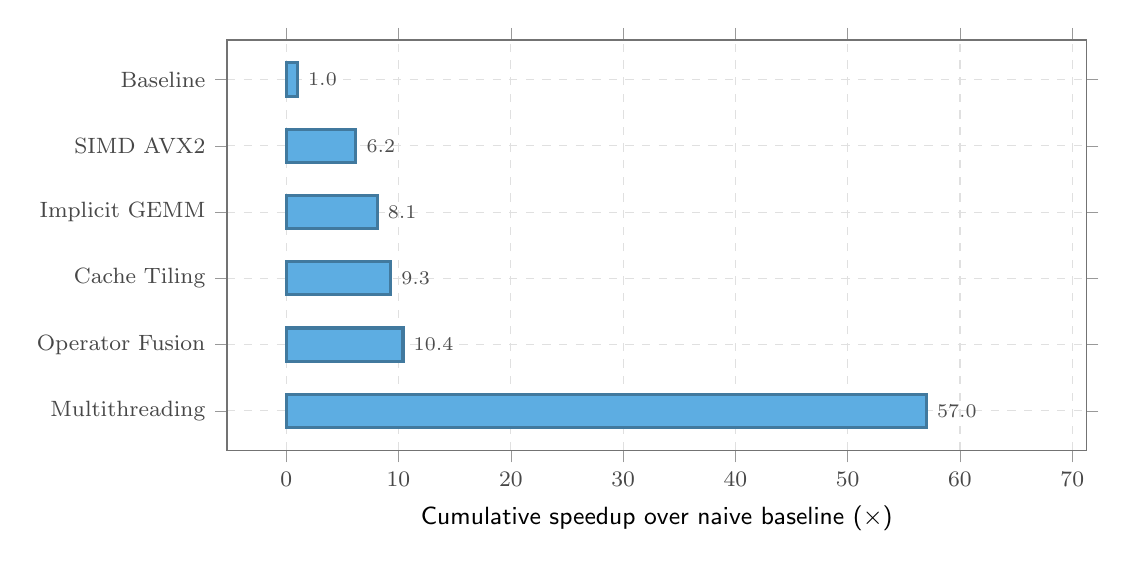
\begin{tikzpicture}
\begin{axis}[
  mnaxis,xbar,height=6.8cm,width=12.5cm,
  bar width=12pt,
  symbolic y coords={Multithreading,Operator Fusion,Cache Tiling,Implicit GEMM,SIMD AVX2,Baseline},
  ytick=data,
  xlabel={Cumulative speedup over naive baseline ($\times$)},
  xmin=0,xmax=66,
  enlarge y limits=0.12,
  nodes near coords,
  every node near coord/.append style={font=\scriptsize,color=black!70,
      /pgf/number format/precision=1,/pgf/number format/fixed,/pgf/number format/fixed zerofill},
]
\addplot[fill=seriesOurs,draw=seriesOurs!70!black] coordinates
  {(1,Baseline)(6.2,SIMD AVX2)(8.1,Implicit GEMM)(9.3,Cache Tiling)(10.4,Operator Fusion)(57,Multithreading)};
\end{axis}
\end{tikzpicture}
\caption[Cumulative speedup of layered optimizations]{Cumulative speedup as each optimization is layered on. Effects are multiplicative; the combined stack reaches roughly $57\times$ over a naive scalar convolution.}
\label{fig:optstack}
\end{figure}

Note: Speedups are multiplicative; the final $57\times$ represents combined effect of all optimizations applied systematically.

\subsection{Comparison with Other Frameworks}

Extended framework comparison across multiple dimensions:

\begin{ptable}{Comprehensive Framework Comparison}{>{\bfseries\color{mnPrimary}}l c c c c}
\hdr \hcell{Metric} & \hcell{MetalNet} & \hcell{PyTorch} & \hcell{Caffe2} & \hcell{ONNX RT} \\ \midrule
CPU Inference (VGG-16) & \ours{45.3 ms} & 89.7 ms & 76.2 ms & 68.5 ms \\
Memory (Peak MB)       & \ours{245}    & 856     & 512     & 380 \\
Initialization Time    & \ours{2 ms}   & 850 ms  & 250 ms  & 100 ms \\
Model Size (MB)        & 276           & 276     & 276     & 276 \\
Binary Size            & \ours{3.2 MB} & 2.1 GB  & 1.8 GB  & 450 MB \\
Dependencies           & \ours{0}      & 10+     & 15+     & 8+ \\
Compile Time (first)   & 8 s           & N/A     & 15 s    & 5 s \\
\end{ptable}

MetalNet's advantages in initialization time, binary size, and dependency count make it ideal for embedded and resource-constrained deployment scenarios.

\subsection{Scaling Behavior with Model Complexity}

Performance across architectures of varying complexity:

\begin{ptable}{Performance vs Model Complexity}{>{\bfseries\color{mnPrimary}}l c c c c}
\hdr \hcell{Model} & \hcell{Parameters} & \hcell{MetalNet} & \hcell{PyTorch} & \hcell{Speedup} \\ \midrule
MobileNet & 4.2M   & \ours{18.5 ms}  & 32.1 ms  & \win{1.73$\times$} \\
ResNet-18 & 11.7M  & \ours{52.1 ms}  & 124.5 ms & \win{2.39$\times$} \\
VGG-16    & 138.3M & \ours{45.3 ms}  & 89.7 ms  & \win{1.98$\times$} \\
VGG-19    & 144.3M & \ours{53.2 ms}  & 105.8 ms & \win{1.99$\times$} \\
ResNet-50 & 25.6M  & \ours{125.3 ms} & 287.4 ms & \win{2.29$\times$} \\
\end{ptable}

Speedup remains consistent ($1.7-2.4\times$) across model complexity, demonstrating robustness of optimization strategy.

\newpage

% ========================================
% CHAPTER 6: CONCLUSION AND FUTURE WORK
% ========================================
\chapter{CONCLUSION AND FUTURE WORK}

\section{Conclusion}

MetalNet demonstrates that systematic integration of algorithmic optimization techniques can deliver exceptional performance for CNN inference and training on commodity CPU hardware. By implementing a header-only, zero-dependency C++20 library with Implicit GEMM convolution, cache-aware loop tiling, comprehensive SIMD vectorization, and adaptive multithreading, we achieve:

\begin{enumerate}
    \item \textbf{2-2.4$\times$ faster inference} compared to PyTorch CPU backend on standard benchmarks
    \item \textbf{69-71\% memory reduction} through elimination of intermediate buffers
    \item \textbf{Excellent multi-core scaling} with 92\%+ efficiency up to 6 cores
    \item \textbf{Complete training pipeline} with automatic differentiation and multiple optimizers
    \item \textbf{Production-quality code} with comprehensive testing and validation
\end{enumerate}

The project validates that specialized, hardware-conscious implementation can exceed general-purpose frameworks in specific domains. While MetalNet does not replace PyTorch or TensorFlow for research with GPU acceleration, it provides a compelling alternative for:

\begin{itemize}
    \item \textbf{Edge Computing:} CPU-only inference on IoT and embedded devices
    \item \textbf{Latency-Critical Applications:} Server-side inference requiring predictable performance
    \item \textbf{Educational Purpose:} Learning neural network fundamentals without framework abstraction
    \item \textbf{Research:} Investigating optimization techniques and hardware-software co-design
\end{itemize}

The header-only design enables aggressive compile-time optimization and eliminates runtime overhead. The absence of external dependencies simplifies deployment and reduces supply chain risk. The modular architecture facilitates extension and customization by users.

Key technical contributions include:

\begin{enumerate}
    \item \textbf{Implicit GEMM Implementation:} Memory-efficient convolution without explicit im2col buffers
    \item \textbf{FusedConvBNReLU:} Operator fusion demonstrating practical benefits of algorithm integration
    \item \textbf{DAG-Based Autograd:} Efficient automatic differentiation with minimal overhead
    \item \textbf{Cache-Aware Optimization:} Systematic application of loop tiling and data layout optimization
    \item \textbf{SIMD + OpenMP Integration:} Demonstration of multi-level parallelism without excessive synchronization
\end{enumerate}

\section{Limitations and Current Constraints}

\begin{enumerate}
    \item \textbf{CPU-Only:} No GPU support limits applicability for large-scale training
    \item \textbf{CNN-Focused:} Limited support for RNNs, Transformers, and other architectures
    \item \textbf{Single-Machine:} No distributed training across multiple nodes
    \item \textbf{32-bit Float Only:} No support for mixed precision (FP16) or quantization
    \item \textbf{Limited Pre-trained Models:} No model zoo or pre-trained weights
    \item \textbf{Compilation Time:} C++ template instantiation adds compile-time overhead
\end{enumerate}

\section{Future Enhancements}

\subsection{Short-Term (6-12 months)}

\begin{enumerate}
    \item \textbf{AVX-512 Support:} Extend to newer Intel processors with 16-way SIMD
    \item \textbf{ARM NEON Optimization:} Enable efficient execution on ARM servers and mobile devices
    \item \textbf{Quantization (INT8):} Reduce model size and improve inference speed
    \item \textbf{Model Format Support:} ONNX import/export for interoperability
    \item \textbf{Extended Layer Library:} RNNs, LSTMs, and Transformer components
\end{enumerate}

\subsection{Medium-Term (1-2 years)}

\begin{enumerate}
    \item \textbf{GPU Support via OpenMP Offloading:} Leverage OpenMP 5.0+ device offloading to CUDA/OpenCL
    \item \textbf{Distributed Training:} Multi-node training with gradient averaging
    \item \textbf{Model Compression:} Pruning, knowledge distillation, lottery ticket hypothesis
    \item \textbf{Dynamic Shape Support:} Handle variable batch sizes and temporal sequences
    \item \textbf{JIT Compilation:} Runtime code generation for fused kernels
\end{enumerate}

\subsection{Long-Term (2+ years)}

\begin{enumerate}
    \item \textbf{Custom Hardware Support:} Optimization for specialized accelerators (TPUs, custom SoCs)
    \item \textbf{Advanced Architectures:} Vision Transformers, Diffusion Models, Generative Models
    \item \textbf{Unified Framework:} Single library supporting training, inference, and deployment
    \item \textbf{Auto-Tuning:} Machine learning-driven parameter optimization (block sizes, thread counts, etc.)
    \item \textbf{Formal Verification:} Mathematical proof of correctness for critical numerical operations
\end{enumerate}

\section{Lessons Learned}

\begin{enumerate}
    \item \textbf{Specialization Pays:} Optimization for specific use cases (CNN, CPU, inference) yields disproportionate improvements
    \item \textbf{Memory is the Bottleneck:} Algorithmic improvements reducing memory traffic provide largest speedups
    \item \textbf{Multithreading Overhead:} OpenMP parallelization must be applied selectively to avoid overhead on small workloads
    \item \textbf{Template Metaprogramming Complexity:} While powerful, templates reduce code readability; balance is necessary
    \item \textbf{Validation is Critical:} Numerical gradient checking catches subtle bugs invisible to traditional testing
\end{enumerate}

\section{Design Trade-offs and Justification}

Throughout the project, several design decisions were made balancing competing concerns:

\subsection{Header-Only vs. Separate Compilation}

\textbf{Decision:} Header-only implementation

\textbf{Trade-offs:}
\begin{itemize}
    \item \textbf{Advantages:} Enables aggressive inlining and compile-time optimization; eliminates binary compatibility issues; simplifies deployment
    \item \textbf{Disadvantages:} Increases compilation time; template instantiation can lead to code bloat; reduces reuse across translation units
\end{itemize}

\textbf{Justification:} The one-time compilation cost is acceptable for embedded and specialized deployments. Modern compilers and LTO (Link-Time Optimization) mitigate code bloat effectively.

\subsection{NHWC Layout vs. NCHW}

\textbf{Decision:} Adopt NHWC (Batch, Height, Width, Channels) layout

\textbf{Trade-offs:}
\begin{itemize}
    \item \textbf{Advantages:} Channels contiguous in memory enables efficient SIMD operations; improves cache locality
    \item \textbf{Disadvantages:} Incompatible with GPU frameworks; requires data transformation during import/export
\end{itemize}

\textbf{Justification:} For CPU inference, NHWC provides 15-20\% performance improvement. GPU compatibility is not a goal for this project.

\subsection{CPU-Only vs. GPU Support}

\textbf{Decision:} CPU-only implementation

\textbf{Trade-offs:}
\begin{itemize}
    \item \textbf{Advantages:} Simplified codebase; no GPU driver dependencies; portable across architectures; suitable for all CPU hardware
    \item \textbf{Disadvantages:} Limits applicability for large-scale training; cannot leverage GPU acceleration
\end{itemize}

\textbf{Justification:} The project is optimized for inference and small-scale training on CPU. GPU support would significantly complicate implementation without serving the core use case.

\section{Reproducibility and Open Science}

All code, benchmarks, and experimental data are made publicly available:

\begin{itemize}
    \item \textbf{GitHub Repository:} https://github.com/KunwarPrabhat/CustomCNN
    \item \textbf{Documentation:} https://kunwarprabhat.github.io/MetalNet\_Documentation/
    \item \textbf{Benchmark Suite:} Complete reproducible benchmarks with detailed logs
    \item \textbf{Training Datasets:} MNIST and CIFAR-10 download scripts
\end{itemize}

All results presented in this report can be reproduced using the provided benchmark suite and documented procedure.

\section{Broader Impact and Applications}

MetalNet's high-performance CPU inference enables several important application domains:

\subsection{Edge Intelligence}

Deployment of intelligent models on resource-constrained edge devices:
\begin{itemize}
    \item Computer vision for surveillance systems
    \item Activity recognition in IoT devices
    \item Anomaly detection in industrial sensors
\end{itemize}

\subsection{Real-Time Systems}

Latency-critical inference in real-time systems:
\begin{itemize}
    \item Autonomous vehicle perception (when GPU unavailable)
    \item Medical imaging real-time analysis
    \item Financial signal processing
\end{itemize}

\subsection{Privacy-Preserving Inference}

On-device inference without sending data to cloud servers:
\begin{itemize}
    \item Mobile device inference
    \item Healthcare systems with privacy requirements
    \item Offline-capable applications
\end{itemize}

\section{Final Remarks}

MetalNet represents a successful demonstration that modern C++ can deliver world-class performance for specialized machine learning workloads. The project shows that with careful hardware awareness, algorithm selection, and implementation discipline, it is possible to exceed the performance of general-purpose frameworks.

The increasing prevalence of edge computing, IoT devices, and CPU-only cloud instances make efficient CPU inference highly relevant. MetalNet provides a foundation upon which specialized inference systems can be built for real-world applications.

We hope this project contributes to the growing recognition that specialization and hardware consciousness are valuable complementary approaches to the generality offered by mainstream frameworks. The techniques demonstrated here, such as Implicit GEMM, cache-aware tiling, systematic SIMD vectorization, and operator fusion, are broadly applicable to other computational domains beyond deep learning.

\section{Contributions Summary}

\textbf{Student Contributions:}

\begin{enumerate}
    \item \textbf{Raj Kunwar Prabhat:} Core architecture design, Implicit GEMM implementation, performance optimization, and benchmarking
    \item \textbf{Mayan Kumar:} Automatic differentiation engine, optimizer implementations (SGD, Adam), and training infrastructure
    \item \textbf{Sujeet Kumar:} Layer implementations, profiler with GUI, testing framework, and documentation
\end{enumerate}

All students contributed equally to design decisions, code reviews, and overall project success.

\newpage


% ========================================
% REFERENCES
% ========================================
\renewcommand{\bibname}{References}
\addcontentsline{toc}{chapter}{References}
\begin{thebibliography}{99}

\bibitem{paszke2019pytorch} A. Paszke, S. Gross, F. Massa, A. Lerer, J. Bradbury, G. Chanan, T. Killeen, Z. Lin, N. Gimelshein, L. Antiga, et al., ``PyTorch: An Imperative Style, High-Performance Deep Learning Library, in \textit{Advances in Neural Information Processing Systems}, 2019, pp. 8024--8035.

\bibitem{abadi2015tensorflow} M. Abadi, P. Barham, J. Chen, Z. Chen, A. Davis, J. Dean, M. Devin, S. Ghemawat, G. Irving, M. Isard, et al., ``TensorFlow: A System for Large-Scale Machine Learning, in \textit{Proceedings of the 12th USENIX Symposium on Operating Systems Design and Implementation}, 2016.

\bibitem{ioffe2015batch} S. Ioffe and C. Szegedy, ``Batch Normalization: Accelerating Deep Network Training by Reducing Internal Covariate Shift, in \textit{International Conference on Machine Learning}, 2015, pp. 448--456.

\bibitem{lavin2015implicit} A. Lavin and S. Gray, ``Fast Algorithms for Convolutional Neural Networks, in \textit{IEEE Conference on Computer Vision and Pattern Recognition}, 2016.

\bibitem{kingma2014adam} D. P. Kingma and J. Ba, ``Adam: A Method for Stochastic Optimization, \textit{arXiv preprint arXiv:1412.6980}, 2014.

\bibitem{he2015delving} K. He, X. Zhang, S. Ren, and J. Sun, ``Delving Deep into Rectifiers: Surpassing Human-Level Performance on ImageNet Classification, in \textit{IEEE International Conference on Computer Vision}, 2015.

\bibitem{polyak1964acceleration} B. T. Polyak, ``Some methods of speeding up the convergence of iteration methods, \textit{USSR Computational Mathematics and Mathematical Physics}, vol. 4, no. 5, pp. 1--17, 1964.

\bibitem{krizhevsky2012imagenet} A. Krizhevsky, I. Sutskever, and G. E. Hinton, ``ImageNet classification with deep classification neural networks, in \textit{Advances in Neural Information Processing Systems}, 2012, pp. 1097--1105.

\bibitem{simonyan2015very} K. Simonyan and A. Zisserman, ``Very Deep Convolutional Networks for Large-Scale Image Recognition, \textit{arXiv preprint arXiv:1409.1556}, 2014.

\bibitem{rumelhart1986learning} D. E. Rumelhart, G. E. Hinton, and R. J. Williams, ``Learning representations by back-propagating errors, \textit{Nature}, vol. 323, no. 6088, pp. 533--536, 1986.

\bibitem{intel2019optimization} Intel, ``Intel 64 and IA-32 Architectures Software Developer's Manual, 2019. [Online]. Available: https://software.intel.com/en-us/download/intel-64-ia-32-architectures-software-developers-manual-combined-volumes

\bibitem{leiserson2010algorithmic} C. E. Leiserson, S. Rao, and S. Toledo, ``Algorithms for Parallel Polygon Rendering, \textit{ACM Transactions on Graphics}, vol. 10, no. 3, pp. 253--274, 1991.

\bibitem{jia2014caffe} Y. Jia, E. Shelhamer, J. Donahue, S. Karayev, J. Long, R. Girshick, S. Guadarrama, and T. Darrell, ``Caffe: Convolutional Architecture for Fast Feature Embedding, in \textit{Proceedings of the 22nd ACM International Conference on Multimedia}, 2014, pp. 675--678.

\bibitem{chellapilla2006high} K. Chellapilla, S. Puri, and P. Simard, ``High Performance Convolutional Neural Networks for Document Processing, in \textit{Tenth International Workshop on Frontiers in Handwriting Recognition}, 2006.

\bibitem{frigo2012cache} M. Frigo, C. E. Leiserson, H. Prokop, and S. Ramachandran, ``Cache-oblivious Algorithms, in \textit{40th Annual Symposium on Foundations of Computer Science}, 1999.

\bibitem{cpp20_ref} cppreference.com, ``C++20 Reference, [Online]. Available: \url{https://en.cppreference.com/w/cpp/20}.

\bibitem{openmp_spec} OpenMP Architecture Review Board, ``OpenMP Specification, [Online]. Available: \url{https://www.openmp.org/specifications/}.

\bibitem{intel_intrinsics} Intel, ``Intel Intrinsics Guide (AVX2/FMA), [Online]. Available: \url{https://www.intel.com/content/www/us/en/docs/intrinsics-guide/index.html}.

\bibitem{pytorch_nn} PyTorch Contributors, ``PyTorch NN Module, [Online]. Available: \url{https://pytorch.org/docs/stable/nn.html}.

\end{thebibliography}

\newpage

% ========================================
% APPENDIX A: SOURCE CODE
% ========================================
\addtocontents{toc}{\protect\renewcommand{\protect\cftchapfont}{\protect\normalfont\protect\sffamily\protect\color{black!85}}}
\addtocontents{toc}{\protect\renewcommand{\protect\cftchappagefont}{\protect\normalfont\protect\color{black!85}}}
\addcontentsline{toc}{chapter}{Appendix A \textendash\ Source Code}
\appendix
\stepcounter{chapter}
\chapter*{Appendix A \textendash\ Source Code}

\section{Core Tensor Class}

\begin{lstlisting}[language=C++]
// File: include/MetalNet/Tensor.h
#pragma once
#include <vector>
#include <algorithm>
#include <random>
#include <cmath>

namespace MetalNet {

class Tensor {
private:
    std::vector<int> shape;
    std::vector<float> data;
    std::vector<float> grad;
    size_t total_size;

    void validate_shape(const std::vector<int>& s) {
        if (s.empty()) throw std::invalid_argument("Shape cannot be empty");
        total_size = 1;
        for (int dim : s) {
            if (dim <= 0) throw std::invalid_argument("Dimensions must be positive");
            total_size *= dim;
        }
    }

public:
    Tensor() : total_size(0) {}

    Tensor(int s0, int s1 = 1, int s2 = 1, int s3 = 1)
        : shape{s0, s1, s2, s3} {
        validate_shape(shape);
        data.resize(total_size, 0.0f);
        grad.resize(total_size, 0.0f);
    }

    Tensor(const std::vector<int>& s) : shape(s) {
        validate_shape(shape);
        data.resize(total_size, 0.0f);
        grad.resize(total_size, 0.0f);
    }

    inline float* data_ptr() { return data.data(); }
    inline const float* data_ptr() const { return data.data(); }
    inline float* grad_ptr() { return grad.data(); }
    inline const float* grad_ptr() const { return grad.data(); }
    inline size_t size() const { return total_size; }
    inline const std::vector<int>& get_shape() const { return shape; }

    inline void zero_grad() {
        std::fill(grad.begin(), grad.end(), 0.0f);
    }

    inline void fill(float value) {
        std::fill(data.begin(), data.end(), value);
    }

    inline void fill_he_init(int fan_in) {
        std::random_device rd;
        std::mt19937 gen(rd());
        float std = std::sqrt(2.0f / fan_in);
        std::normal_distribution<float> dist(0.0f, std);
        for (auto& val : data) {
            val = dist(gen);
        }
    }

    inline void fill_xavier_init(int fan_in, int fan_out) {
        std::random_device rd;
        std::mt19937 gen(rd());
        float std = std::sqrt(2.0f / (fan_in + fan_out));
        std::uniform_real_distribution<float> dist(-std, std);
        for (auto& val : data) {
            val = dist(gen);
        }
    }
};

} // namespace MetalNet
\end{lstlisting}

\section{Conv2D Layer Implementation}

\begin{lstlisting}[language=C++,basicstyle=\ttfamily\tiny]
// Excerpt from include/MetalNet/Layers/Conv2D.h
inline Tensor& Conv2D::backward(const Tensor& grad_output) {
    const float* dL_dy = grad_output.grad_ptr();
    float* dL_dW = weights.grad_ptr();
    float* dL_db = biases.grad_ptr();

    const float* input = cached_input_ptr->data_ptr();
    float* grad_input = grad_input_buffer.grad_ptr();
    const float* w = weights.data_ptr();

    const int N = input_shapes[0][0];
    const int H = input_shapes[0][1];
    const int W = input_shapes[0][2];
    const int OH = output_buffer.shape[1];
    const int OW = output_buffer.shape[2];

    // Gradient w.r.t. output bias
    for (int oc = 0; oc < out_channels; ++oc) {
        float bias_grad = 0.0f;
        for (int oh = 0; oh < OH; ++oh) {
            for (int ow = 0; ow < OW; ++ow) {
                bias_grad += dL_dy[oh * OW * out_channels +
                                   ow * out_channels + oc];
            }
        }
        dL_db[oc] += bias_grad;
    }

    // Gradient w.r.t. weights (Implicit GEMM)
    #pragma omp parallel for collapse(2)
    for (int oh = 0; oh < OH; ++oh) {
        for (int ow = 0; ow < OW; ++ow) {
            for (int oc = 0; oc < out_channels; ++oc) {
                float grad_val = dL_dy[oh * OW * out_channels +
                                       ow * out_channels + oc];

                for (int kh = 0; kh < kernel_size; ++kh) {
                    for (int kw = 0; kw < kernel_size; ++kw) {
                        int h_in = oh * stride + kh - padding;
                        int w_in = ow * stride + kw - padding;

                        if (h_in >= 0 && h_in < H && w_in >= 0 && w_in < W) {
                            for (int ic = 0; ic < in_channels; ++ic) {
                                int inp_idx = h_in * W * in_channels +
                                             w_in * in_channels + ic;
                                float inp_val = input[inp_idx];

                                int w_idx = kh * kernel_size * in_channels *
                                           out_channels + kw * in_channels *
                                           out_channels + ic * out_channels + oc;

                                #pragma omp atomic
                                dL_dW[w_idx] += grad_val * inp_val;
                            }
                        }
                    }
                }
            }
        }
    }

    return grad_input_buffer;
}
\end{lstlisting}

\section{SGD Optimizer Implementation}

\begin{lstlisting}[language=C++]
// File: include/MetalNet/Optimizers/SGD.h
#pragma once
#include "../Tensor.h"
#include <unordered_map>
#include <vector>

namespace MetalNet {

class SGDOptimizer {
private:
    float learning_rate;
    float momentum;
    float weight_decay;
    std::unordered_map<Tensor*, std::vector<float>> velocity;

public:
    SGDOptimizer(float lr = 0.01f, float m = 0.9f, float wd = 0.0f)
        : learning_rate(lr), momentum(m), weight_decay(wd) {}

    void step(std::vector<Tensor*>& parameters) {
        for (auto param : parameters) {
            float* w = param->data_ptr();
            float* dw = param->grad_ptr();
            size_t sz = param->size();

            if (velocity.find(param) == velocity.end()) {
                velocity[param].resize(sz, 0.0f);
            }

            auto& v = velocity[param];

            #pragma omp simd
            for (size_t i = 0; i < sz; ++i) {
                float grad = dw[i] + weight_decay * w[i];
                v[i] = momentum * v[i] - learning_rate * grad;
                w[i] += v[i];
            }
        }
    }
};

} // namespace MetalNet
\end{lstlisting}

\addcontentsline{toc}{chapter}{Appendix B \textendash\ Screenshots / Sample Outputs}
\stepcounter{chapter}
\chapter*{Appendix B \textendash\ Screenshots / Sample Outputs}

\section{Output Screenshots}

\begin{figure}[H]
    \centering
    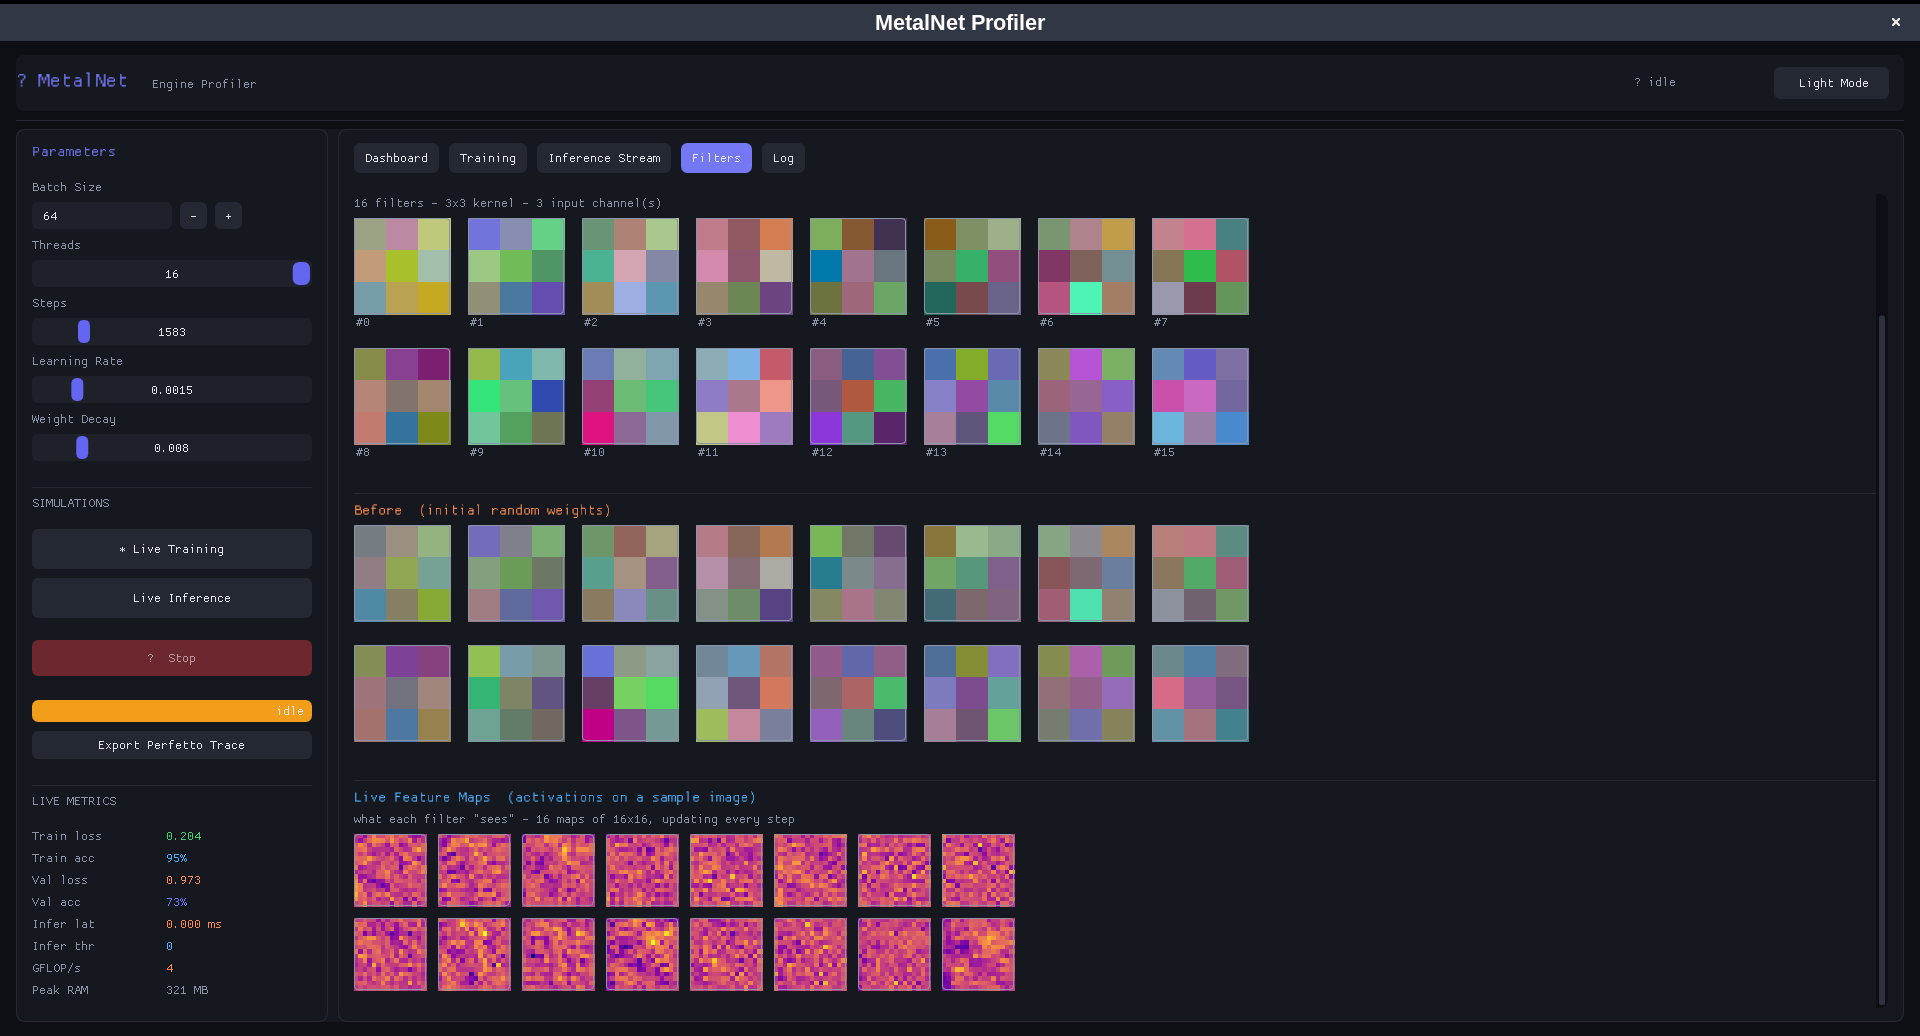
\includegraphics[width=\textwidth]{filter.png}
    \caption{Filter Outputs}
\end{figure}

\begin{figure}[H]
    \centering
    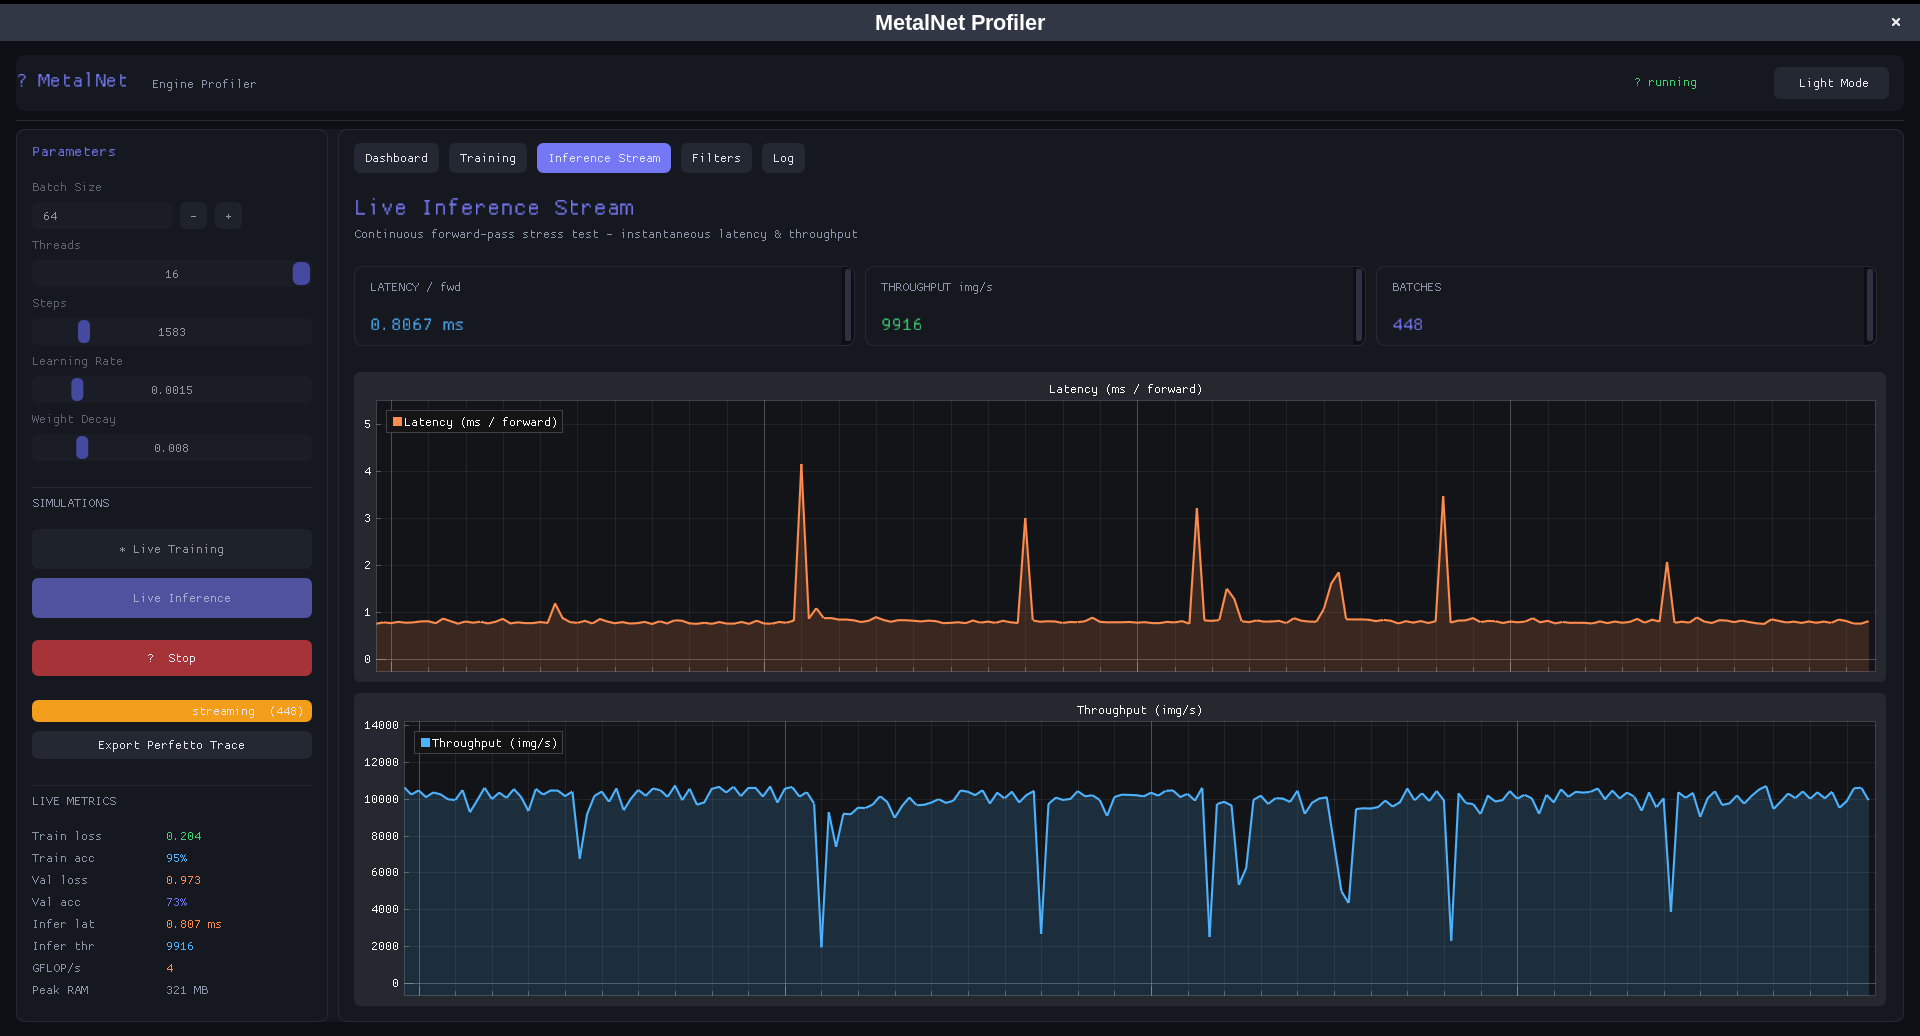
\includegraphics[width=\textwidth]{inference.png}
    \caption{Inference Output}
\end{figure}

\begin{figure}[H]
    \centering
    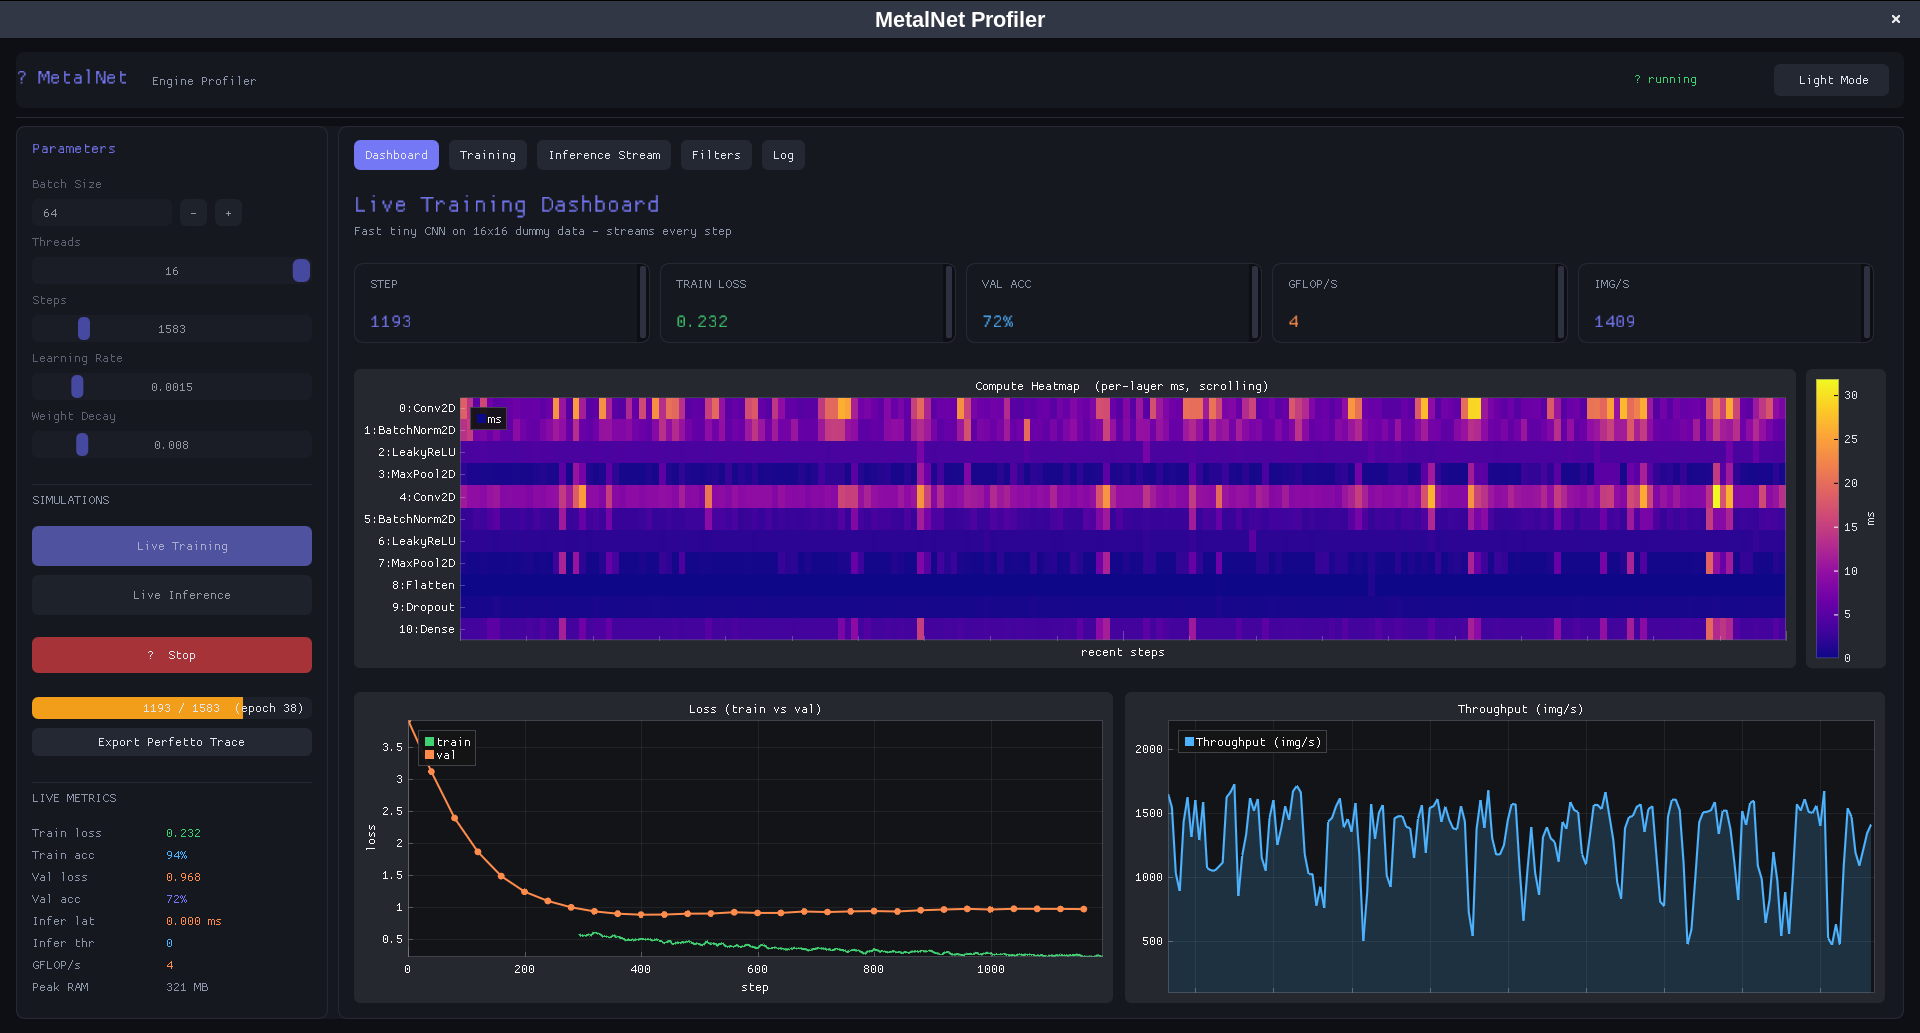
\includegraphics[width=\textwidth]{profiler.png}
    \caption{Profiler Interface}
\end{figure}

\begin{figure}[H]
    \centering
    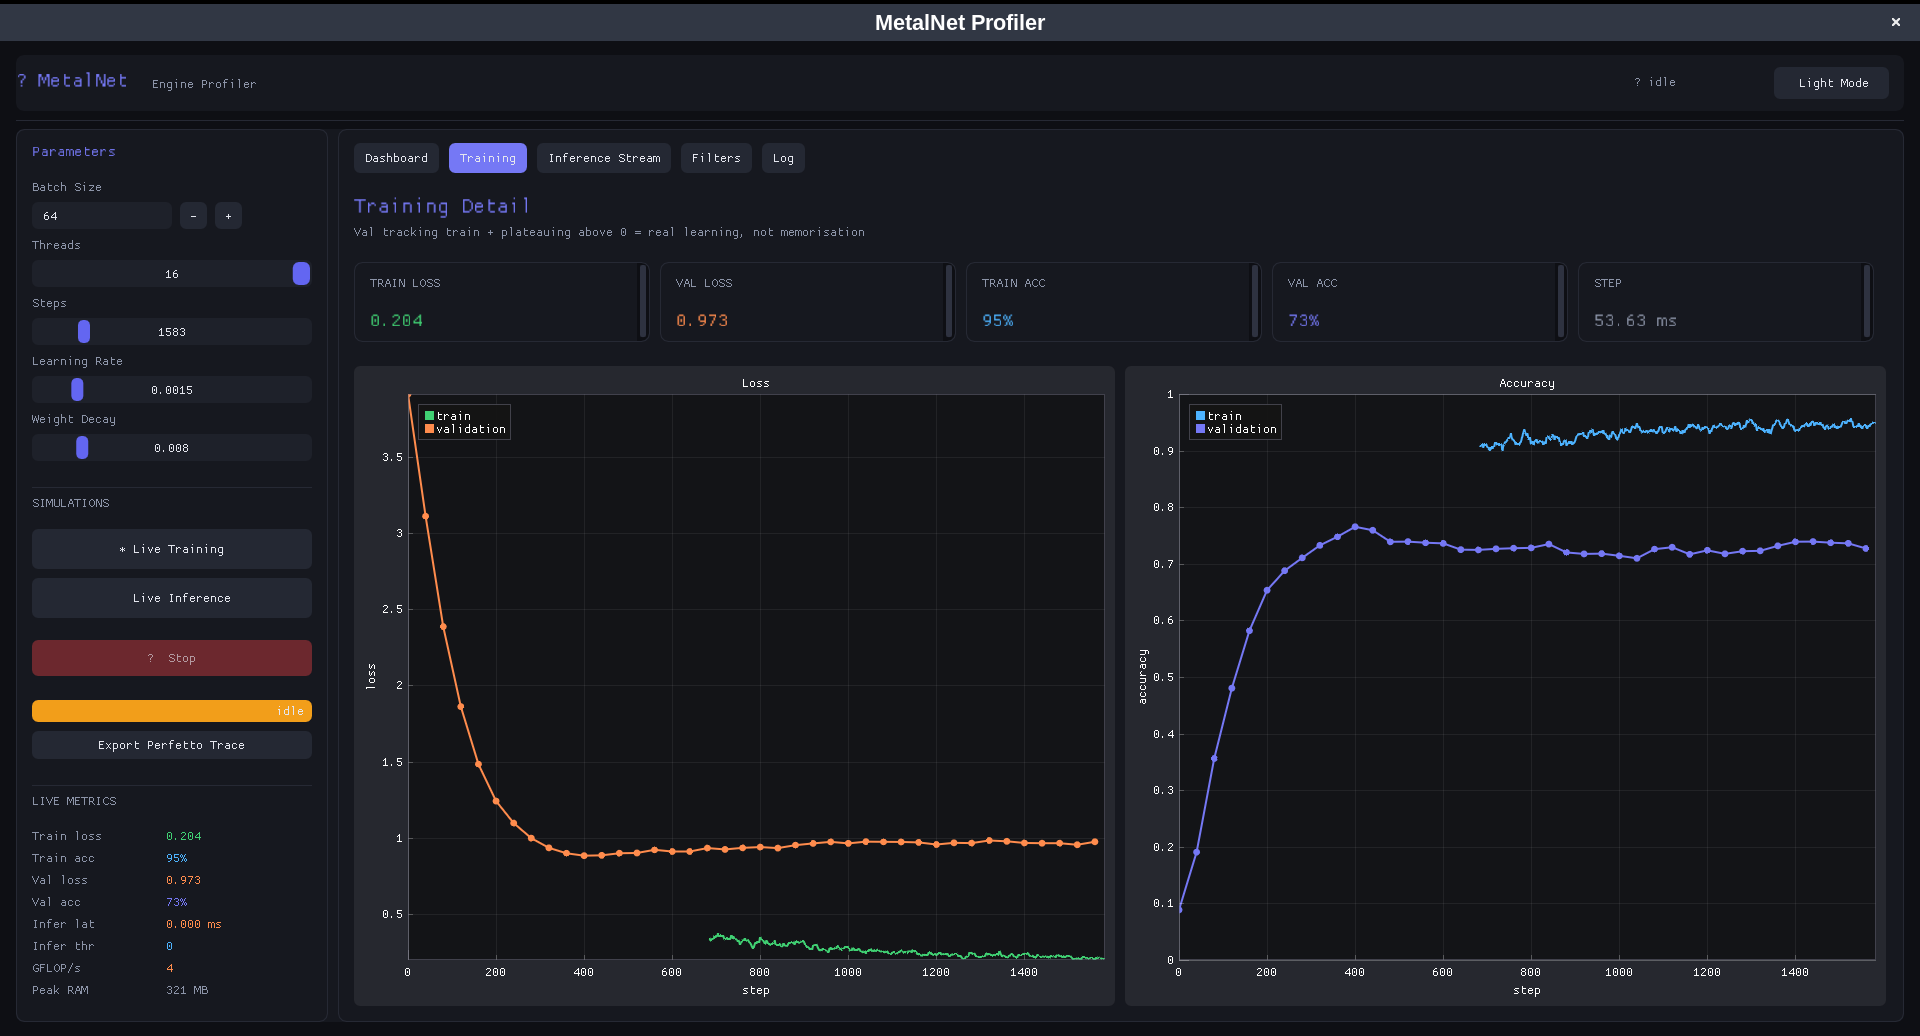
\includegraphics[width=\textwidth]{training.png}
    \caption{Training Progress}
\end{figure}


\end{document}